\chapter{Dusty Quasars} \label{Dust}

In this chapter we aim to identify the type of dust extinction present in the observed population of quasars and to construct de-reddened quasar SEDs for a subset of the Sloan Digital Sky Survey's (SDSS) 7th data release (DR7) quasar catalog \citep{Schneider:2010}.  By distinguishing between objects that are intrinsically red and those that are dust reddened, we can also comment on the broad emission \citep[e.g., ][]{Richards:2003} and broad absorption line \citep[e.g., ][]{Reichard:2003a,Reichard:2003b} properties of quasars as a function of their intrinsic color (and the amount of dust reddening).  These emission line properties can help to reveal the SED shape outside of the range covered by our data, as a function of the masses, and/or inclinations that correlate with intrinsic color.
To this end this chapter is structured as follows:  \S\ref{sec:model} focuses on the identification and fitting of various dust reddening models including individual reddening values for each quasar in our sample. We analyze composite spectra as a function of these fitted values in \S\ref{sec:spectra} and present our conclusions in \S\ref{sec:conclusions}. The data used throughout this chapter are presented in \S\ref{Dust_data}.

\section{Fitting Reddening Models to Quasar Photometry} \label{sec:model}

\begin{figure*}%[ht]
\begin{center}
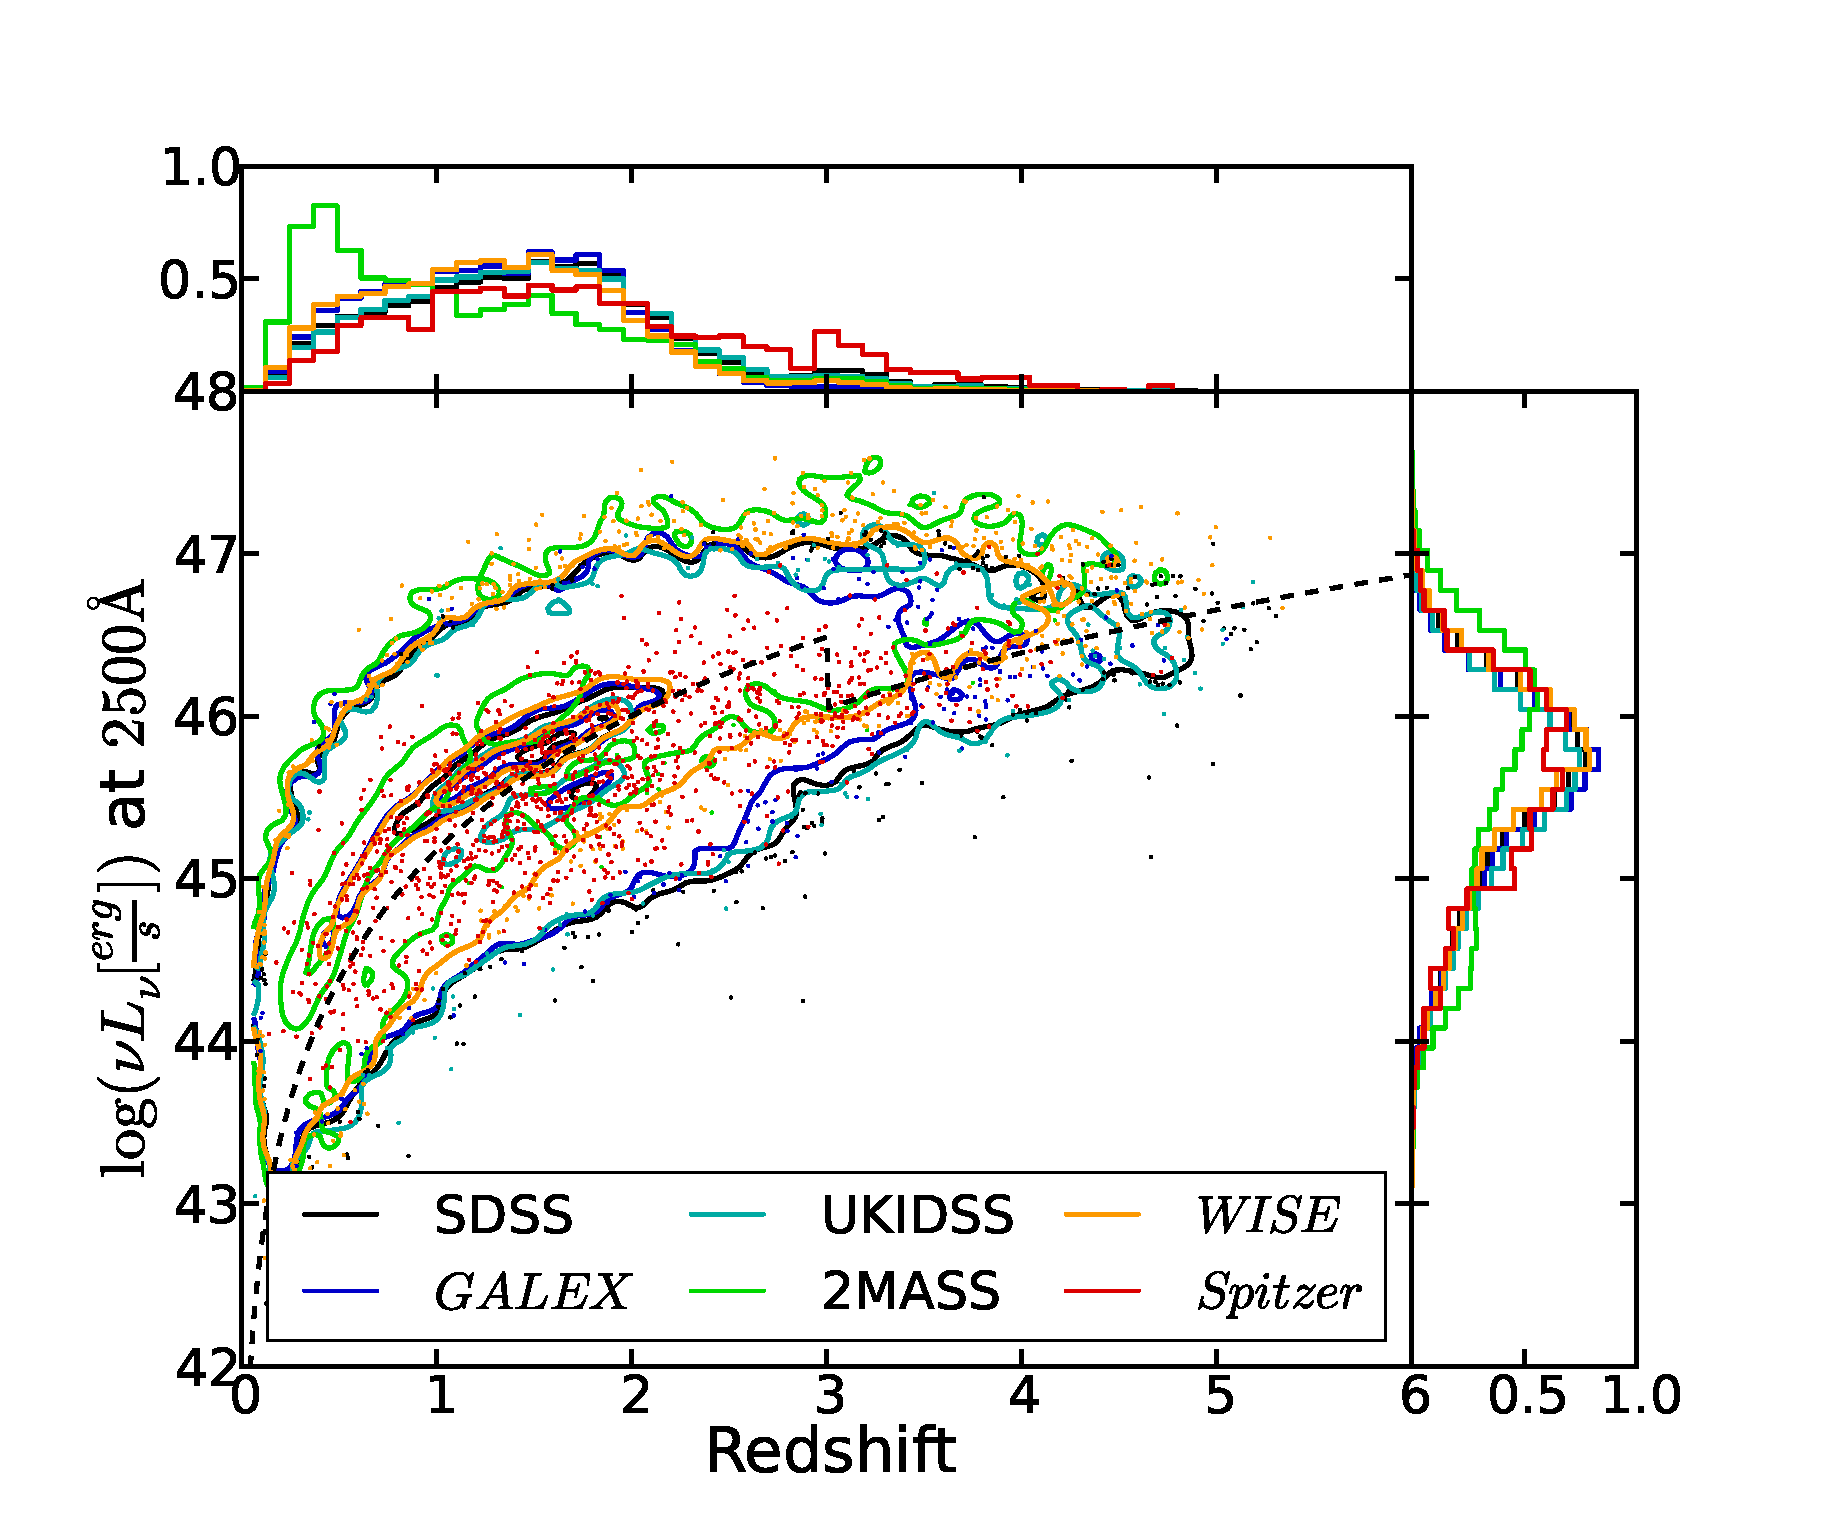
\includegraphics[width=6.25in]{images/Dust/f2}
\caption[Colors vs. redshift]{\label{fig:mode} Colors as a function of redshift with the modes indicated by the red lines.  The colors indicate the linear density of points with white being most dense and the outliers shown as black points. The vertical dashed lines indicate the redshift where each color passes into the Ly$\alpha$ line.}
\end{center}
\end{figure*}

\subsection{Modal Colors}

To identify a quasar as ``red,'' we must first determine both
the expected distribution of SEDs and a method for identifying which
quasars can be considered as outliers from that distribution.
The expected observed SED changes as a function of redshift as the different spectral lines are shifted though the filter sets.  By examining quasar colors as a function of redshift we can find the typical quasar SED, and assuming this SED contains little or no dust, we can use it to characterize the effects that different reddening laws have on the SED. However, we note that these colors are calculated after removing the estimated host galaxy contribution (most relevant at z$\lesssim$0.8) using the prescription discussed in Chapter~\ref{SEDs}.

Previous studies have mitigated against emission lines changing a quasar's colors by binning the data by redshift and removing the median \citep[e.g.,][]{Richards:2003} or mode \citep[e.g.,][]{Hopkins:2004} within each bin. The results of this process are strongly dependent of the bin width chosen.  To avoid this issue, we used a non-parametric \nth{2} degree local regression to estimate the modal color as a function of redshift.  We used the \texttt{loess} regression package in \texttt{R} with smoothing parameters chosen so the regression followed the ridge-line (i.e. the mode) for each color-redshift plot, as in Figure~\ref{fig:mode}.  Although this method does not work well once a filter passes into the Lyman forest 
%(e.g. $u-g$ for $z\gtrsim2$)
(vertical dashed lines in Figure~\ref{fig:mode}), with the rest frame wavelength cuts applied in the analysis, this discrepancy does not affect our results.

\begin{figure*}%[ht]
\begin{center}
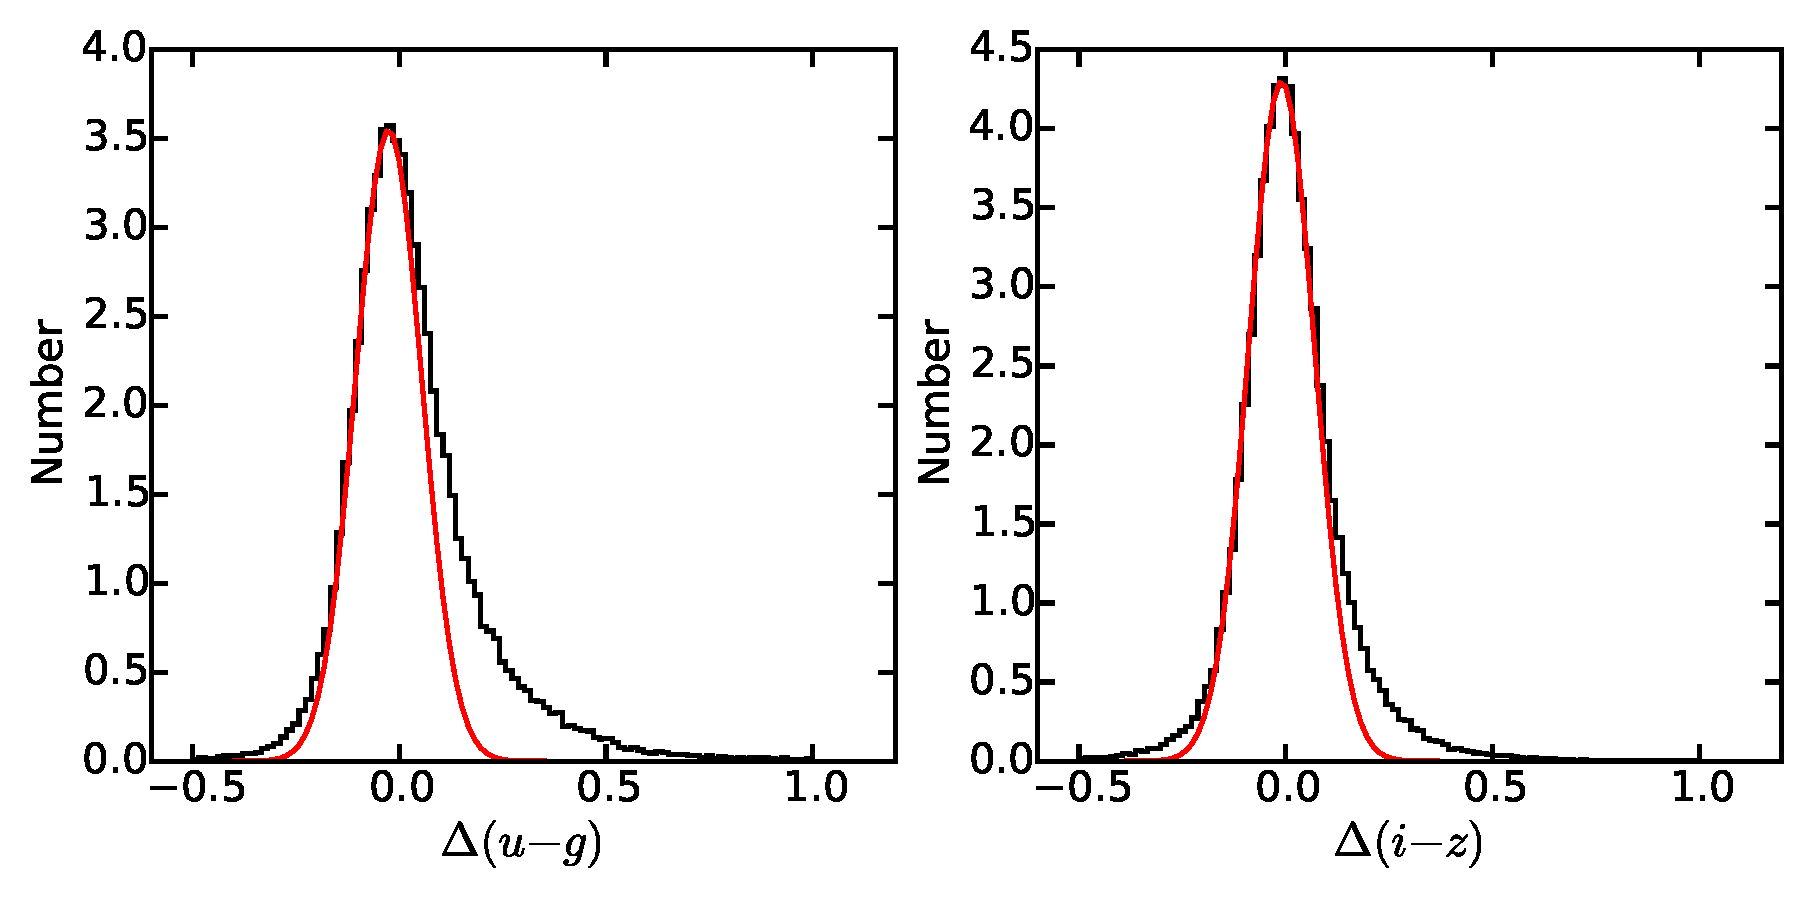
\includegraphics[width=6.25in]{images/Dust/f3}
\caption[Relative colors]{\label{fig:Dug} 
%Relative colors. 
Relative colors for $\dug$ ({\em left}) and $\diz$({\em right}). $\dug$ shows a heavy red tail as compared to its best fit Gaussian (red), while $\diz$ shows a weaker red tail as compared to its best fit Gaussian. This asymmetry indicates that there is a population of dust reddened quasars in our sample.}
\end{center}
\end{figure*}

With these modal colors, we define relative colors \citep{Richards:2003} as the difference between the observed color and the modal color at the quasar's redshift (e.g. $\dug=(u-g)-\langle u-g \rangle_{{\rm mode},z}$).  From these relative colors we can also build relative magnitudes ($\mrel$) up to a normalization factor; we adopt $\mrel_{i{\rm band}}=0$ throughout this paper.  These relative colors and magnitudes allow for a color analysis that is independent of emission line effects.
%for which it is possible to make fair comparisons of different colors.

To determine if we have a population of quasars affected by dust reddening, we compare the distributions for a relative color on the blue end of the quasar SED ($\dug$) and and relative color on the red end of the quasar SED ($\diz$).  If there is no dust reddening in our population, we would expect the shape of these two distributions to be the same, whereas dust reddening would cause there to be (relatively) more red quasars on the blue end of the SED than the red end of the SED.  Thus we can distinguish between dust reddening and synchrotron emission extending to the optical since dust preferentially absorbs the shorter-wavelength photons (e.g. adding a heavy red tail to $\dug$), while synchrotron adds long-wavelength photons (e.g. adding a heavy red tail to $\diz$).  Figure~\ref{fig:Dug} shows these two distributions and we can see $\dug$ shows a heavier red ``tail'' than $\diz$, indicating that we do indeed have a population of dust reddened quasars.


\subsection{Red vs. Reddened: Photometry} \label{sec:red_v_red:phot}

As discussed in \citet{Richards:2003}, ``red" quasars can be intrinsically red or dust reddened.  In order to tell these two apart, we need to understand how dust changes the observed $\mrel$.  Combining Equation~\ref{eqn:red_eq} with our definition of $\mrel$ and assuming the modal quasar contains no dust\footnote{This technically measures dust reddening relative to the modal quasar and is in addition to any reddening of the modal quasar itself.}:
\begin{align} \label{eqn:rel_red_eq} 
\mrel&=m - \langle m \rangle_{{\rm mode},z} &&{\rm  (observed)} \nonumber \\
&=m_0 + 2.5\dal \log{(\lambda)} + \ebv R_\lambda &&{\rm  (model)}
\end{align}
where $m_0$ is a normalization term, $\dal$ is the difference between the quasar's {\em intrinsic} spectral index and the {\em observed} modal spectral index of $\alpha_{\lambda} =-1.72$ ($\alpha_{\nu}=-0.28$, as determined from the modal colors in Figure~\ref{fig:mode}), with positive values being bluer, and $R_{\lambda}$ is a function dependent on the properties of the dust.  Throughout the remainder of the chapter we will be working with values of 2.5$\dal$ since that is the term that appears in the model.  These values can be converted to absolute spectral indices ($f_{\lambda} \propto \lambda^{\alpha_{\lambda}}$, $f_{\nu} \propto \nu^{\alpha_{\nu}}$) by adding in the observed modal spectral index:
\begin{eqnarray}
	\alpha_{\lambda} &=& -1.72 - \dal \label{eqn:dal_2_al} \\
	\alpha_{\nu} &=& -2-\alpha_{\lambda} \nonumber \\
	&=& -0.28 + \dal \label{eqn:dal_2_anu}
\end{eqnarray}

\begin{figure}[t]
\begin{center}
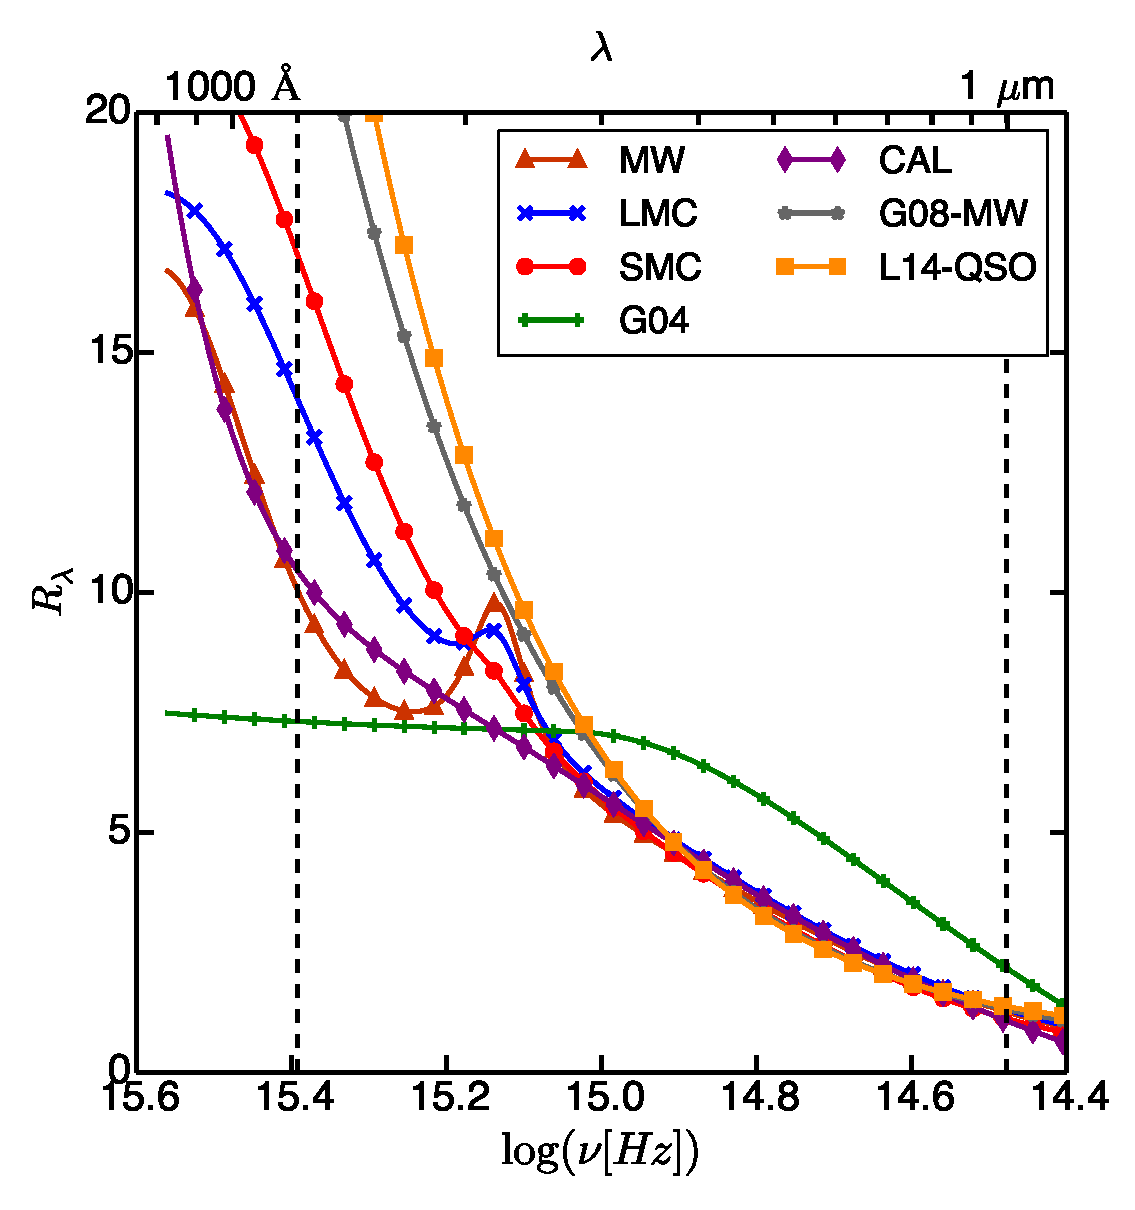
\includegraphics[width=4.5in]{images/Dust/f4}
\caption[Dust extinction curves]{ \label{fig:ecurves} Extinction curves for seven different reddening laws with $\ebv=1$: Milky Way type (brown triangles), LMC type (blue X's), SMC type (red dots), starburst type (purple diamonds), \citet{Goobar:2008} type (grey stars), \citet{Leighly:2014} type (orange squares), and \citet{Gaskell:2004} type (green +'s). The vertical dashed lines indicate the polynomial fitting range used in this chapter. In all cases we see dust reddening adds curvature to the relative magnitudes.}
\end{center}
\end{figure}

As stated in \S\ref{sec:dust_intro}, this model only holds between 1\,$\mu$m and 1216\,\AA, since that is where the underlying SED is well approximated by a single powerlaw.  The one thing $R_{\lambda}$ has in common across all forms of dust is that it adds {\em curvature} to $\mrel$ by preferentially removing shorter wavelength photons (except for \citealt{Gaskell:2004} reddening which introduces curvature in the opposite sense).
%preferentially removes shorter wavelength photons \textbf{[GTR: except Gaskell]}, effectively adding   
Figure~\ref{fig:ecurves} shows $R_{\lambda}$ for seven different reddening laws with $\ebv=1$:  Milky Way \citep[MW;][]{Pei:1992}, Large Magellanic Cloud \citep[LMC;][]{Pei:1992}, Small Magellanic Cloud \citep[SMC;][]{Pei:1992}, starburst \citep[CAL;][]{Calzetti:1995}, multiple-scattering dust fit to the Milky Way \citep[G08-MW;][]{Goobar:2008}, multiple-scattering dust fit to a BAL quasar \citep[L14-QSO;][]{Leighly:2014}, and \citet[G04;][]{Gaskell:2004} type reddening.

\begin{figure*}%[ht]
\begin{center}
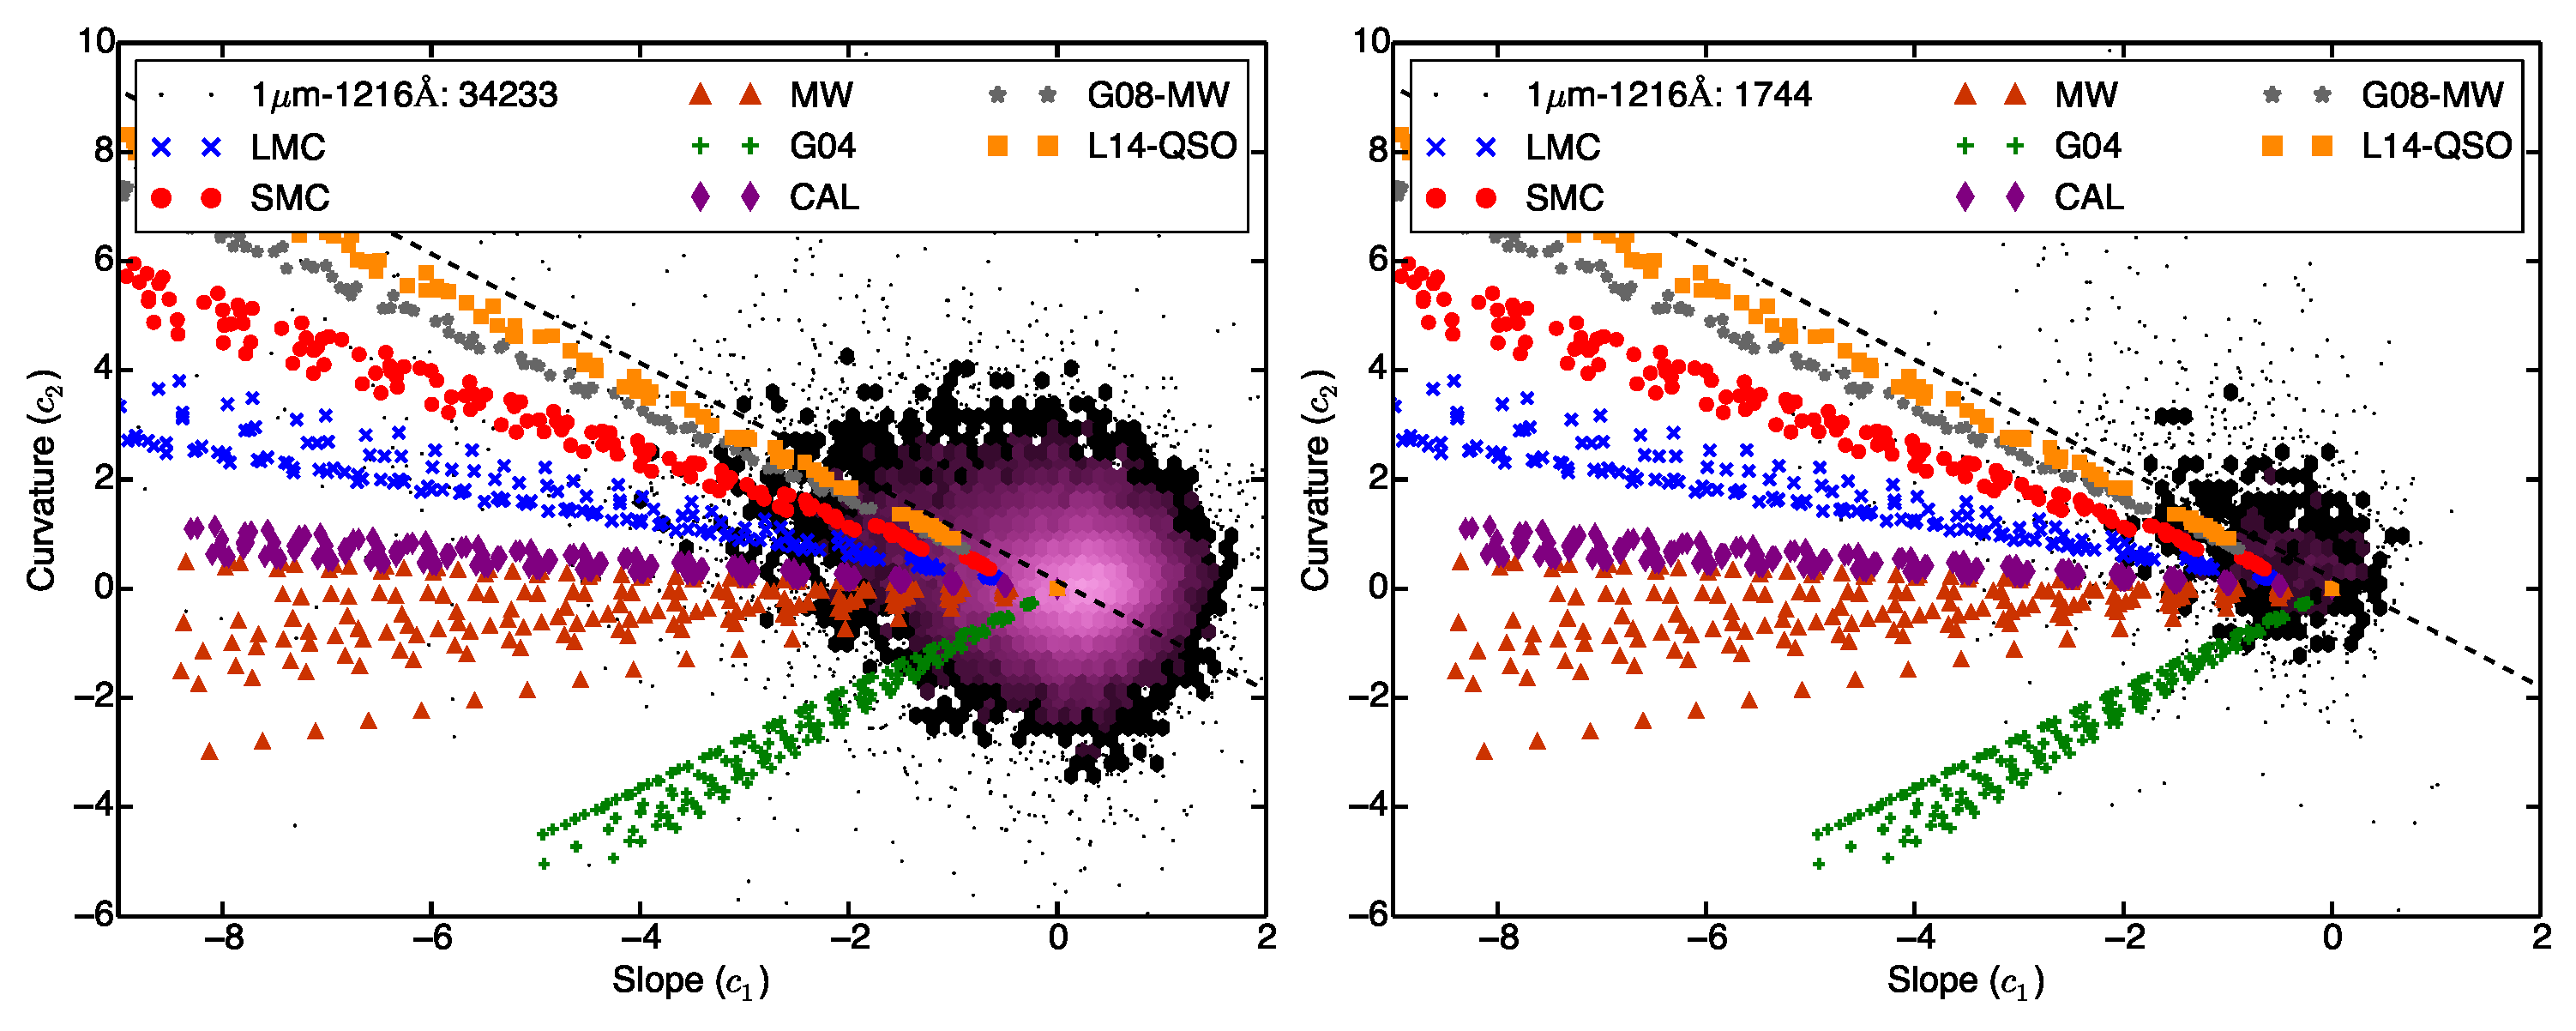
\includegraphics[width=6.2in]{images/Dust/f5}
\caption[$c_1$ vs. $c_2$]{ \label{fig:c1c2} $c_1$ vs. $c_2$ for uniformly selected SDSS quasars.  The colors indicate the linear density of scatter points with white being the most dense and the outliers are shown as black scatter points.  The symbols show a typical quasar placed at redshifts ranging from 0--2.2 and with $\ebv$ values ranging from 0--0.8 for seven different reddening laws: SMC type (red dots), LMC type (blue X's), starburst type (purple diamonds), Milky Way type (brown triangles), multiple-scattering dust fit to the Milky Way \citep[grey stars][]{Goobar:2008}, multiple-scattering dust fit to a BAL quasar \citep[orange squares][]{Leighly:2014}, and \citet{Gaskell:2004} type (green +'s).  The black dashed line shows the orthogonal regression of the data.  {\em Left}: Sample of 34,233 non-BAL quasars. {\em Right}: Sample of 1,744 BAL quasars.  In both samples the trend of the data best matches the steeper reddening laws.}
\end{center}
\end{figure*}

From Equation~\ref{eqn:rel_red_eq} we see that changes in the intrinsic spectral index ($\dal$) will change the slope of $\mrel$ (i.e. it is only multiplied by $\log{(\lambda)}$), while changes in the amount of dust ($\ebv$) will change both the slope and curvature of $\mrel$ since $R_{\lambda}$ contains higher orders of $\log{(\lambda)}$.  \citet{Hopkins:2004} characterized these changes by fitting $\mrel$ with a \nth{1}-order Chebyshev polynomial to obtain the slope ($c_1$), and fitting $\mrel$ with a \nth{2}-order Chebyshev polynomial to obtain the curvature ($c_2$).  Because of the orthogonality properties of the Chebyshev polynomials, $c_1$ and $c_2$ are linearly independent of each other.  This property means that changes in a quasar's intrinsic spectral index will {\em only} change $c_1$, but given the nature of $R_{\lambda}$, changes in $\ebv$ will change {\em both} $c_1$ and $c_2$.

Figure~\ref{fig:c1c2}  shows the $c_1$ vs. $c_2$ parameter space for both the non-BAL ({\em left}) and BAL ({\em right}) samples, where the symbols show the modal quasar ($c_1$=0, $c_2$=0 by definition) reddened by seven different reddening laws with redshifts ranging from 0--2.2 and $\ebv$ values ranging from 0--0.8. If the reddening were instead applied to a quasar that was intrinsically blue (red) then the symbols would shift to higher (lower) $c_1$ values while the $c_2$ values would remain unchanged.  Looking at the trend of the BAL and non-BAL quasar samples in Figure~\ref{fig:c1c2}, it appears that the data is most closely matched with the steeper reddening laws, e.g., the SMC dust law or the multiple-scattering dust model described by \citet{Goobar:2008} to explain anomalous dust extinction in supernovae host galaxies \citep[see also][]{Fynbo:2013,Leighly:2014}.

\subsection{Monte Carlo Parameter Estimation} \label{sec:mcmc}
One of the difficulties of our analysis is the degeneracy between changes in color and dust reddening \citep[e.g., ][]{Richards:2003,Reichard:2003a,Reichard:2003b}.  As such, to fit for both the individual 2.5$\dal$ and $\ebv$ values along with the shapes of the distributions they come from, we use a multi-level or hierarchical Bayesian model.  In our model we assume the 2.5$\dal$ values come from a normal distribution with mean $\mu_\alpha$ and width $\sigma_\alpha$ and the $\ebv$ values come from an exponentially modified Gaussian (EMG) distribution.  The EMG is the result of summing a normal random variable with mean $\mu_{\rm dust}$ and width $\sigma_{\rm dust}$ and an exponential random variable with rate parameter $\lambda_{\rm dust}$ (smaller values indicate a heavier red tail).  The EMG was chosen since it is very similar in shape to the half-normal, half-exponential distribution \citet{Hopkins:2004} found to work well for the $\ebv$ distribution of quasars. In addition to these parameters we also assume a noise term with zero mean and width $S$ to model error in determining the modal colors.
The technical details of this process are included in Appendix~\ref{ch:mcmc} for the interested reader; we summarize the results in \S\ref{sec:mcmc_results} and continue our analysis in \S\ref{sec:spectra}.  

\begin{figure*}
\begin{center}
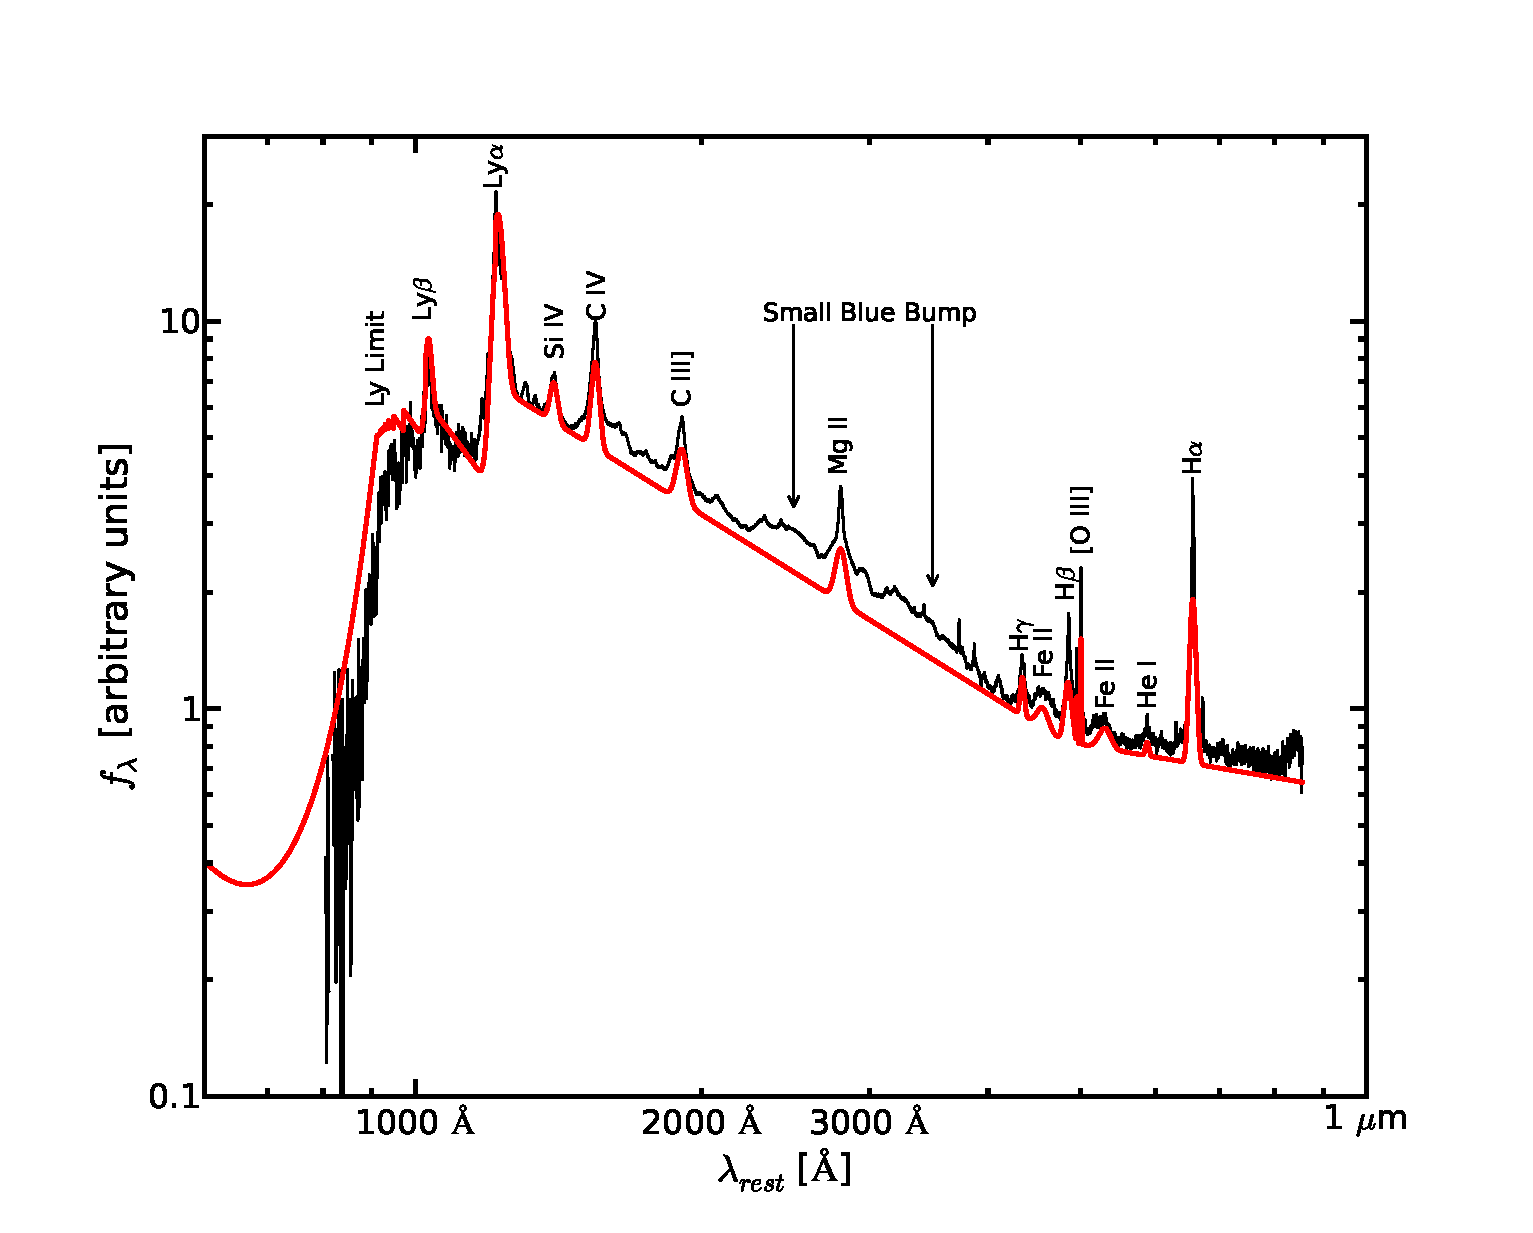
\includegraphics[width=6.25in]{images/Dust/f6}
\caption[Best fit population parameters for non-BAL quasars]{\label{fig:mcmc_no_bal_tri} The best fit population parameters for an SMC reddening law for the non-BAL quasars. The red dashed lines show the median for each variable, the 1$\sigma$ (2$\sigma$) confidence regions are shown in green (orange).  The 2.5$\dal$ distribution is fit with a normal distribution with mean $\mu_{\alpha}$ and width $\sigma_{\alpha}$. The $\ebv$ distribution is fit with a EMG with shape parameters $\mu_{\rm dust}$, $\sigma_{\rm dust}$, and $\lambda_{\rm dust}$ (see text). $S$ is the uncertainty associated with determining the $\mrel$.  
The mean values for these parameters are: $\{ \mu_{\alpha}, \sigma_{\alpha}, \mu_{\rm dust}$, $\sigma_{\rm dust} ,\lambda_{\rm dust}, S \}=\{ 0.169,0.466,-0.0184,7\times10^{-5},31.03,0.0490 \}$.
In the left column, third from the top, we see a positive correlation between the mean values of the 2.5$\dal$ and $\ebv$ distributions, showing there is a degeneracy between these variables.}
\end{center}
\end{figure*}

\begin{figure*}
\begin{center}
\includegraphics[width=6.25in]{images/Dust/f8}
\caption[Best fit population parameters for BAL quasars]{\label{fig:mcmc_bal_tri} Same as Figure~\ref{fig:mcmc_no_bal_tri} but for the BAL quasars. 
The mean values for these parameters are: $\{ \mu_{\alpha}, \sigma_{\alpha}, \mu_{\rm dust}$, $\sigma_{\rm dust} ,\lambda_{\rm dust}, S \}=\{ 0.269,0.516,0.0111,5.2\times10^{-4},22.71,0.0755 \}$.
As with the non-BAL sample we find a positive correlation between the mean values of the 2.5$\dal$ and $\ebv$ distributions, showing there is a degeneracy between these variables.  The BAL sample has a larger value for $\mu_\alpha$ and a smaller value for $\lambda_{\rm dust}$ than the non-BAL sample, indicating that the BAL quasars, on average, are intrinsically bluer within random error (see text) and have more dust reddening than the non-BAL sample.}
\end{center}
\end{figure*}

\subsection{MCMC Results: Population Parameters} \label{sec:mcmc_results} 

Using the model described in \S\ref{sec:mcmc_model}, we fit for both individual 2.5$\dal$ 
%\footnote{see Equations~\ref{eqn:dal_2_al} and \ref{eqn:dal_2_anu} for conversion to absolute spectral indices} 
and $\ebv$ values ($\phi_i=\{2.5\dal_i, \ebv_i \}$ from Appendix~\ref{ch:mcmc}) and the population parameters ($\theta=\{ \mu_{\alpha}, \sigma_{\alpha}, \mu_{\rm dust}$, $\sigma_{\rm dust} ,\lambda_{\rm dust}, S \}$ from Appendix~\ref{ch:mcmc}) describing the distributions of these variables.  This method was used for both the SMC reddening law and the multiple-scattering reddening law from \citet{Goobar:2008} calibrated to fit Mark 231 \citep[a BAL quasar;][]{Leighly:2014}.  The resulting values of the population parameters for both reddening laws are given in Table~\ref{tab:hyp_fit_table} (see also the top and side panels of Figures~\ref{fig:indv_fits_SMC} and \ref{fig:indv_fits_L14}). Figures~\ref{fig:mcmc_no_bal_tri} and~\ref{fig:mcmc_bal_tri} show the marginalized posterior distributions for the 1D and 2D projections for each of the six population parameters for the non-BAL and the BAL samples using the SMC reddening law\footnote{The results for the L14-QSO fit are qualitatively similar.}. 

\begin{deluxetable}{lrrrrr}
\tablewidth{0pt}

\tablecaption{\label{tab:hyp_fit_table} Hyperparameter Fit Values}
\tablehead{
\colhead{} & \multicolumn{2}{c}{SMC} & \colhead{} & \multicolumn{2}{c}{L14-QSO} \\
\cline{2-3} \cline{5-6} \\
\colhead{Population Parameter} & \colhead{non-BAL} & \colhead{BAL} & \colhead{} & \colhead{non-BAL} & \colhead{BAL}
}
\startdata
$\mu_{\alpha}\tablenotemark{a}$      & $0.169\pm0.004\phantom{0}$                 & $0.269^{+0.022\phantom{00}}_{-0.021}$      & & $0.098\pm0.004\phantom{0}$               & $0.052^{+0.019\phantom{00}}_{-0.018}$ \\
$\sigma_{\alpha}\tablenotemark{a}$ & $0.466\pm0.003\phantom{0}$                 & $0.516^{+0.019\phantom{00}}_{-0.018}$      & & $0.505\pm0.003\phantom{0}$               & $0.535\pm0.015$ \\
$\mu_{\rm dust}$                                   & $-0.0184\pm0.0001$                                  & $0.0111^{+0.0009\phantom{0}}_{-0.0007}$ & & $-0.0125\pm0.0001$                               & $0.0007^{+0.0004\phantom{0}}_{-0.0003}$\\
$\sigma_{\rm dust}$                              & $0.00007^{+0.00005}_{-0.00004}$         & $0.00052^{+0.00051}_{-00030}$                   & & $0.0004\pm0.0001$                                 & $0.00027^{+0.00023}_{-00015}$ \\
$\lambda_{\rm dust}\tablenotemark{b}$ & $31.03^{+0.16\phantom{000}}_{-0.18}$ & $22.71^{+0.48\phantom{000}}_{-0.52}$         & & $53.96^{+0.31\phantom{000}}_{-0.27}$ & $41.53^{+0.89\phantom{000}}_{-0.81}$\\
$S$                                                          & $0.0490\pm0.0002$                                    & $0.0755\pm0.0014$                                           & & $0.0469\pm0.0002$                                    & $0.0671\pm0.0012$
\enddata
\tablenotetext{a}{These are the shape parameters for 2.5$\dal$ not $\alpha_{\lambda}$.}
\tablenotetext{b}{Smaller values indicate a heavier tail.}

\tablecomments{The 1$\sigma$ error regions are given for each value.}
\end{deluxetable}

These projections reveal information about the overall shapes of our 2.5$\dal$ and $\ebv$ distributions and correlations between the population parameters.  Both samples have a positive value for $\mu_{\alpha}$ indicating that the (intrinsic) mean spectral indices are bluer than the observed modal quasar ($\dal \gtrsim 0.07$).
For the SMC law the BAL sample is bluer ($\langle \alpha_\lambda \rangle = -1.83$) than the non-BAL sample ($\langle \alpha_\lambda \rangle = -1.79$).
%, and for the L14-QSO law the BAL sample is slightly redder ($\langle \alpha_\lambda \rangle = -1.74$) than the non-BAL sample ($\langle \alpha_\lambda \rangle = -1.76$).  
Although the values of $\mu_\alpha$ are different in terms of random error, after taking into account our systematic ability to measure the modal spectral index (related to $S$, see Appendix~\ref{sec:mcmc_model}), these values are well within 1$\sigma$ of each other (see the top panel of Figure~\ref{fig:indv_fits_SMC}). This indicates that the non-BAL and BAL quasar spectral indices are consistent with coming from the same distribution.
%statistically different between the two samples, these differences are within 1--2$\sigma$ of our (systematic) ability to measure the modal spectral index (related to $S$), indicating that the non-BAL and BAL quasars are consistent with having the same mean spectral index for both reddening laws.

\begin{figure*}[t]
\begin{center}
\begin{tabular}{c}
	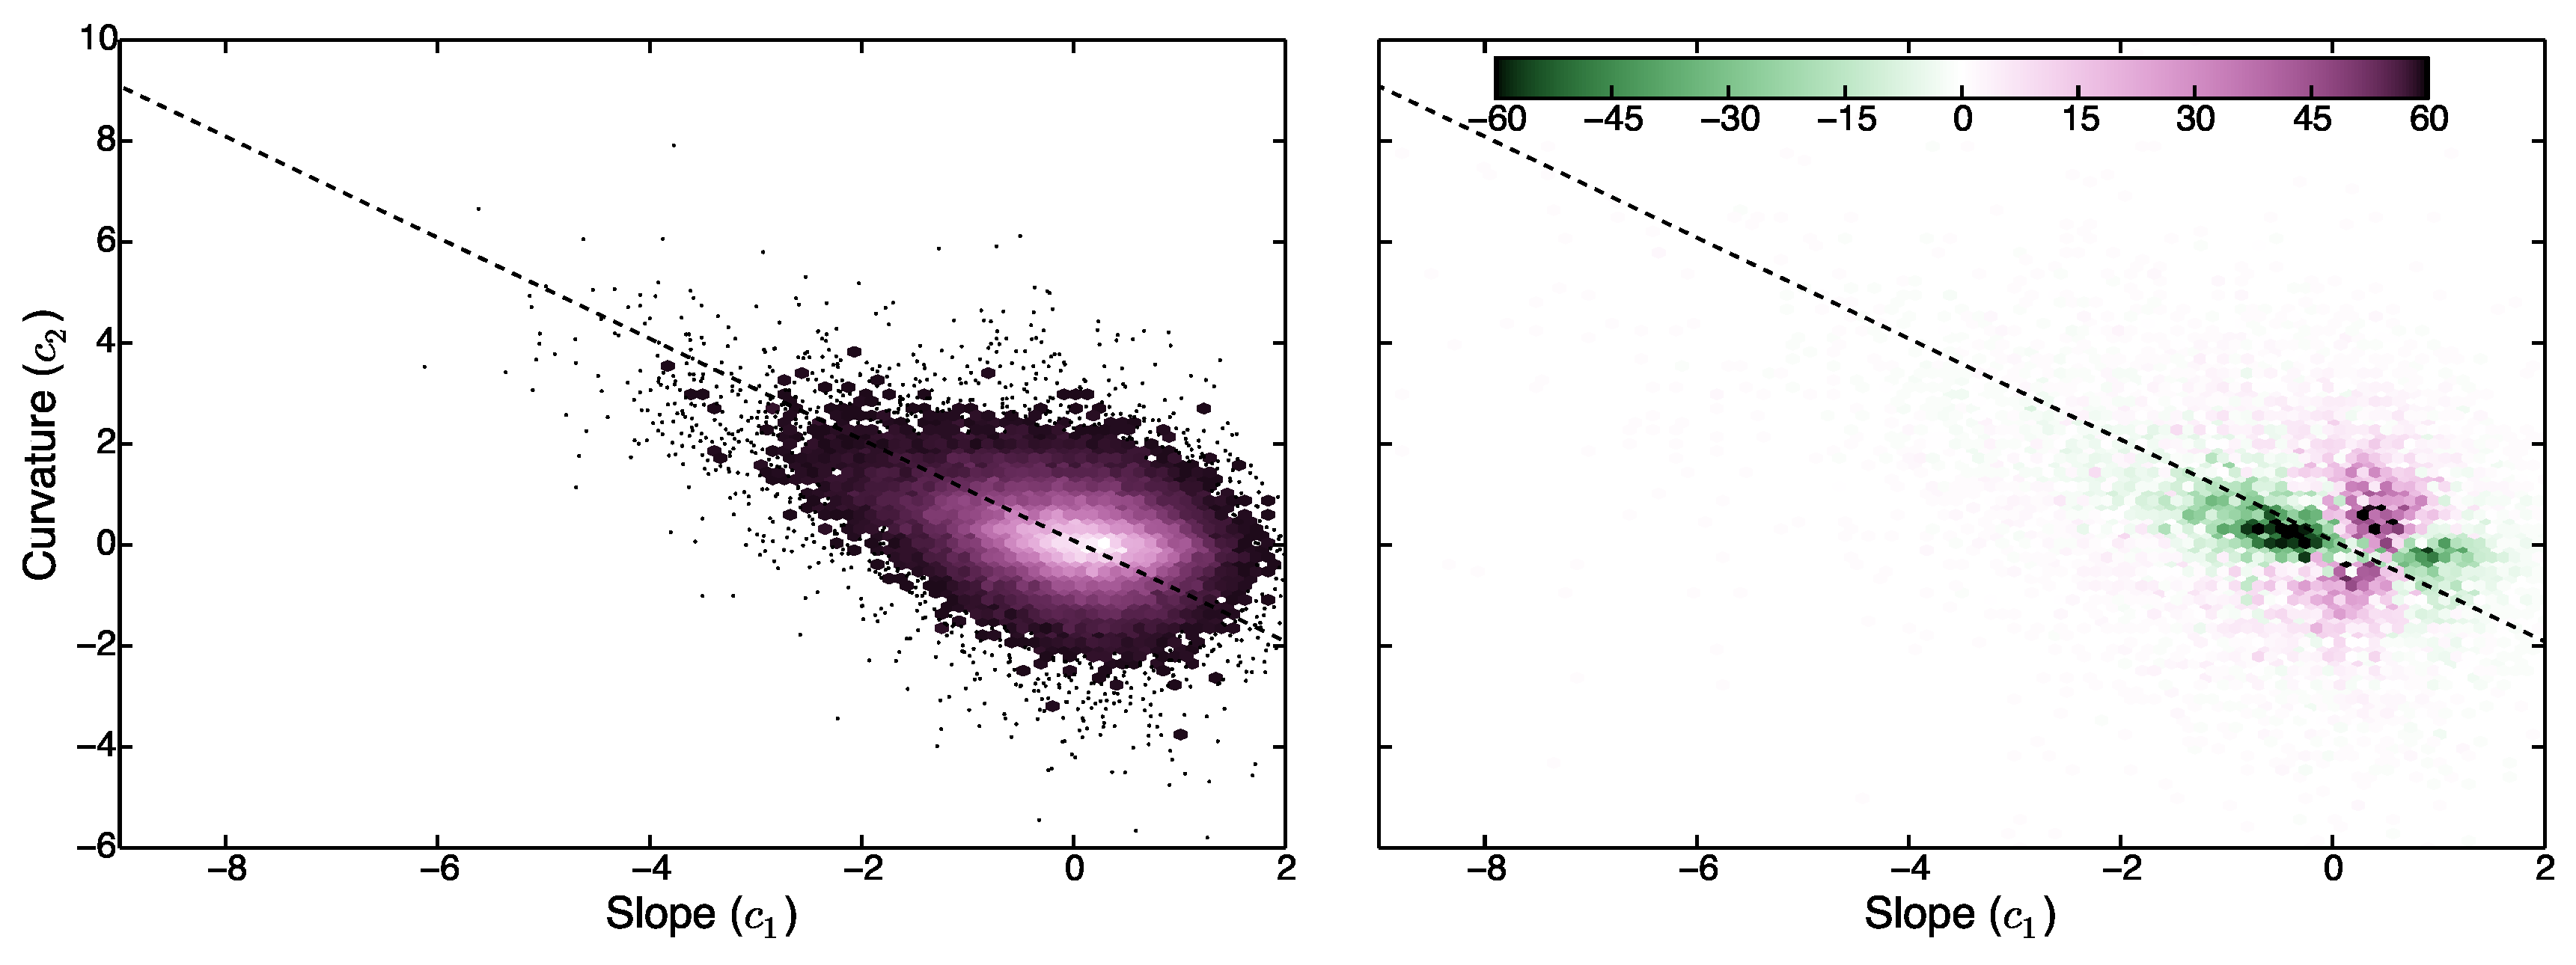
\includegraphics[width=6.25in]{images/Dust/f7} \\
	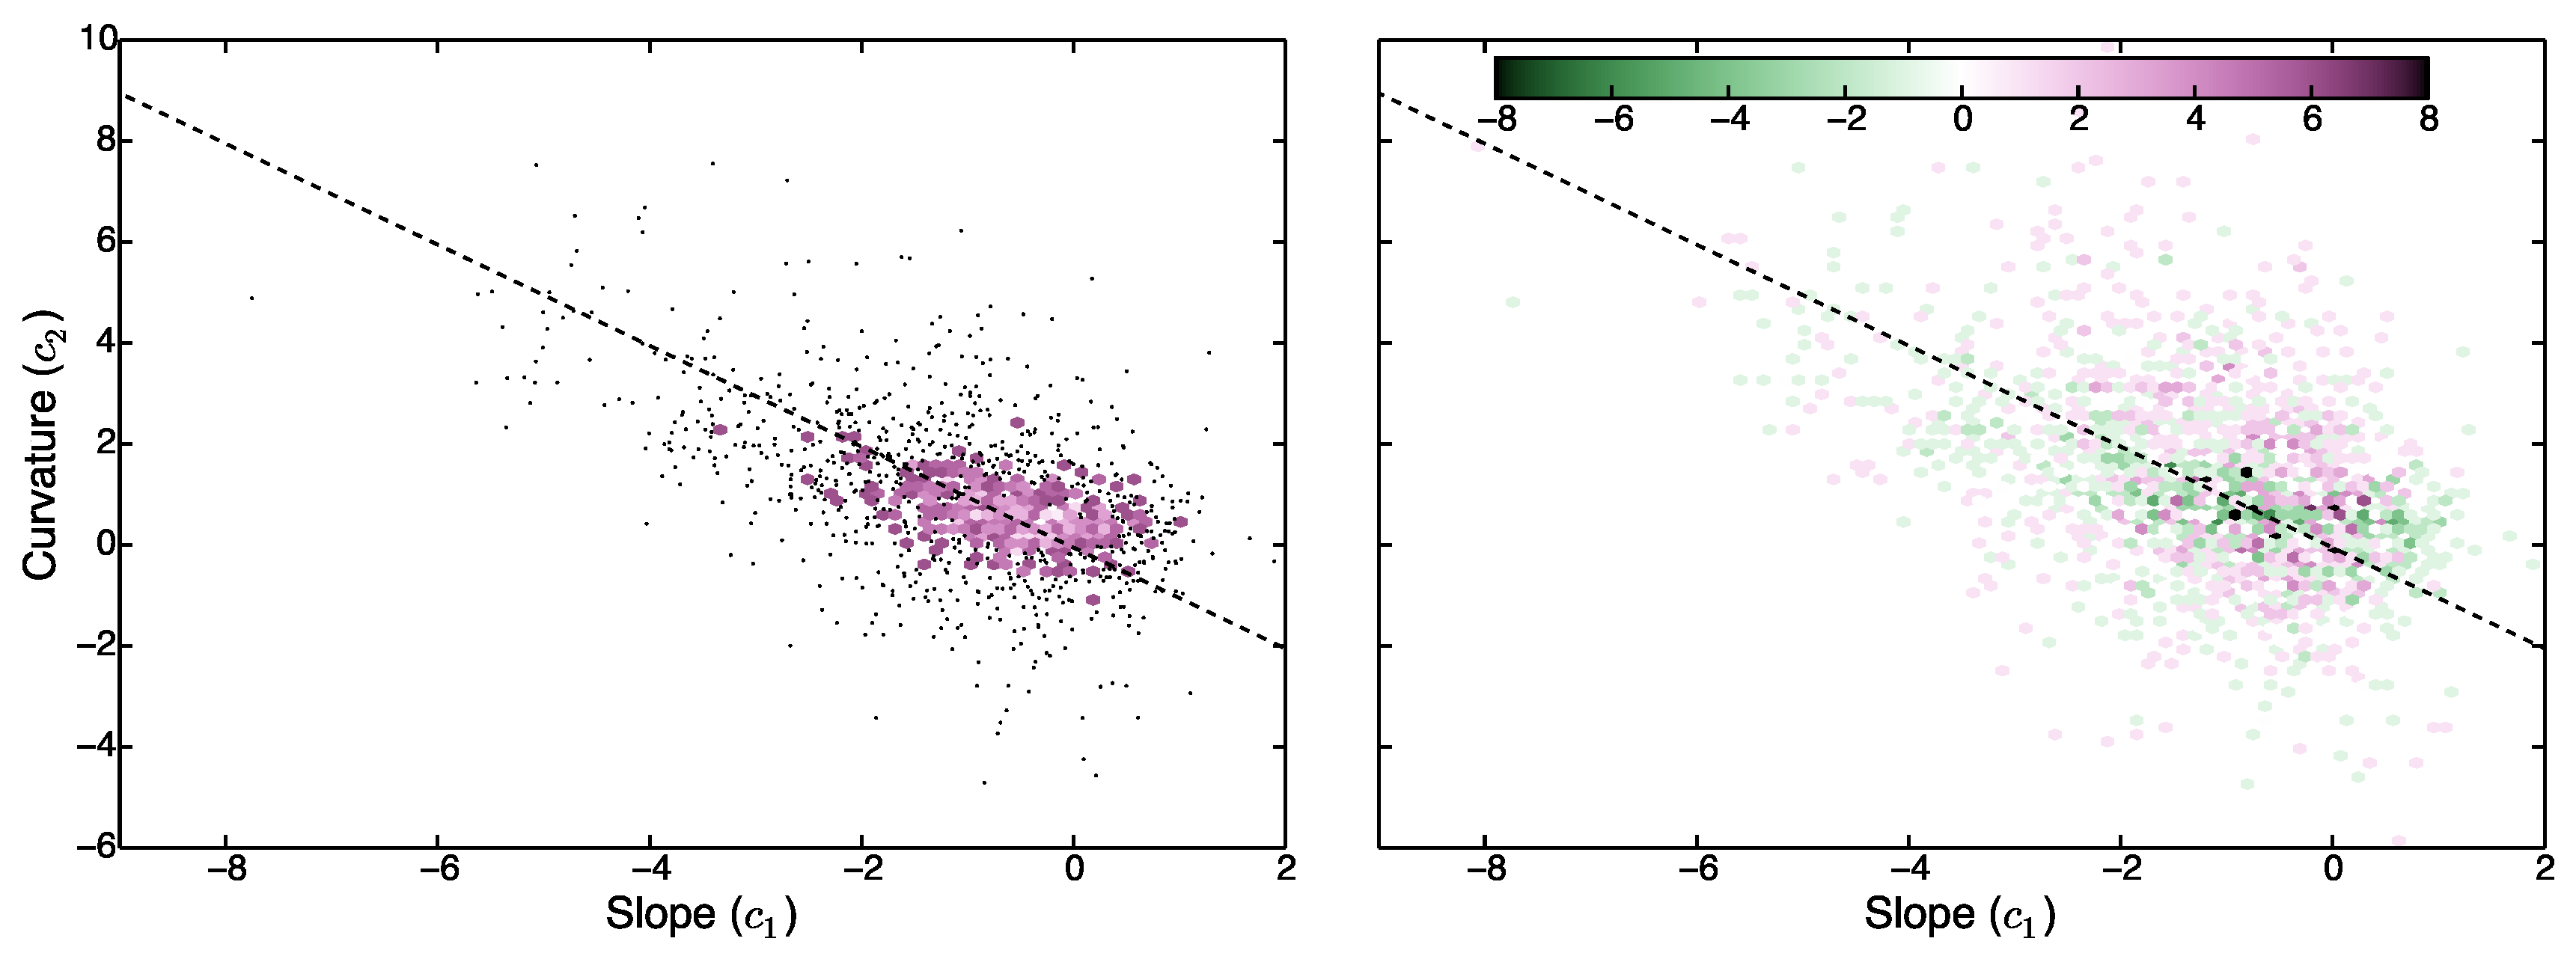
\includegraphics[width=6.25in]{images/Dust/f9}
\end{tabular}
\caption[$c_1$ vs. $c_2$ for MC sample of non-BAL quasars]{\label{fig:mcmc_no_bal_mc} 
Monte Carlo simulations of $c_1$ and $c_2$ ({\em left}) and residuals with the data ({\em right}) for the SMC reddening law based on the population parameters shown in Figures~\ref{fig:mcmc_no_bal_tri} \& \ref{fig:mcmc_bal_tri} for the non-BAL ({\em top}) and BAL ({\em bottom}) samples. The orthogonal regression for the MC distributions are shown as a black dashed line in each panel.
Our model over-predicts the number of quasars with low curvature, indicating it is likely under-predicting the amount of dust in the sample or that the powerlaw model is not a perfect representation of the continuum.}
\end{center}
\end{figure*}

In all cases $\sigma_{\rm dust}$ is consistent with $0$; since this parameter corresponds to the width of the Gaussian half of the EMG distribution, this means the distribution for $\ebv$ is consistent with coming from a pure exponential distribution that is offset from the origin by $\mu_{\rm dust}$.  We also find a positive correlation between $\mu_{\alpha}$ and $\mu_{\rm dust}$ (left column, third from the top in Figures~\ref{fig:mcmc_no_bal_tri} \& \ref{fig:mcmc_bal_tri}) showing there is a degeneracy between the mean values for $\dal$ and $\ebv$ in the model.
That is, it is difficult to distinguish between something that is intrinsically red and something that is dust reddened. 
The positive value of $\mu_{\rm dust}$ in the BAL sample suggests that all of the BAL quasars are consistent with having dust reddening, while the negative value on the non-BAL sample suggests that there are quasars ($\sim$60\%\footnote{Within 1$\sigma$ of 0}) with no dust reddening\footnote{If the modal quasar has a small amount of dust reddening, negative $\ebv$ values would indicate quasars with less dust than the mode.}.

Our population parameters for the SMC law are comparable to the shape parameters found in Table~2 of \citet{Hopkins:2004}. After converting the parameters to the same scale ($\sigma_{\alpha}^{\rm Hopkins} = \sigma_{\alpha}/2.5$, $\sigma_{\rm dust}^{\rm Hopkins} = 1/\lambda_{\rm dust}$, and $\sigma_{\rm Gaussian}^{\rm Hopkins}=\sigma_{\rm dust}$) we find $\sigma_{\alpha}$ (0.33 in Hopkins) to be higher for the non-BAL (0.47) and BAL (0.52) samples, indicating we see a larger range of spectral indices,
and $\lambda_{\rm dust}$ (22.22 in Hopkins) to be about the same for the BAL sample (22.71) and higher\footnote{Higher values mean fewer reddened quasars} for the non-BAL sample (31.03).  As mentioned above, our values for $\sigma_{\rm dust}$ are much smaller than the \citet{Hopkins:2004} value of 0.02.

To check how well our model can recreate the observed data
%To see how well these population parameters represent our data 
we simulate an MC sample of quasars using the results of our fit to find $c_1$ and $c_2$ values.  The resulting distributions can be seen in the left panels of Figure~\ref{fig:mcmc_no_bal_mc} while right panels show the residual with the original data. In the residual plots, green shows where the model over-estimated and purple shows where it under-estimated the number of objects.  In Figure~\ref{fig:mcmc_no_bal_mc} we see that the model over-predicts the number of objects along the direction of largest deviation in $c_1$--$c_2$ space, whereas along the direction perpendicular (with the smallest deviation in $c_1$--$c_2$ space), the model under-predicts the number of objects.  This difference shows that our model favors changes in the slope over changes curvature, and as a result under-estimates the amount of curvature in our data.  This is not surprising given that the average object has low curvature.  This difference could also be attributed to the underlying SED not being well modeled by a powerlaw.  In the bottom right panel of Figure~\ref{fig:mcmc_no_bal_mc} the agreement for the BAL sample is better, but again the amount of curvature is under-estimated by our model.

\setlength{\tabcolsep}{4pt}

\begin{deluxetable}{lcccccccccccccccccc}
\tabletypesize{\scriptsize}
\tablewidth{0pt}

\tablecaption{\label{mean_sed_table} Mean Quasar SEDs }
\tablehead{ \colhead{}  &\colhead{}  &\colhead{}  &\multicolumn{2}{c}{} &\multicolumn{2}{c}{} &\multicolumn{2}{c}{} &\multicolumn{2}{c}{\ion{C}{4} Line} &\multicolumn{2}{c}{\ion{C}{4} Line} &\multicolumn{2}{c}{} &\multicolumn{2}{c}{} &\multicolumn{2}{c}{} \\
\colhead{$\log{(\nu)}$}  &\colhead{All}  &\colhead{$\sigma_{\textup{All}}$}  &\multicolumn{2}{c}{Low Lum.} &\multicolumn{2}{c}{Mid Lum.} &\multicolumn{2}{c}{High Lum.} &\multicolumn{2}{c}{Zone 1} &\multicolumn{2}{c}{Zone 2} &\multicolumn{2}{c}{UV Bump} &\multicolumn{2}{c}{Scott UV} &\multicolumn{2}{c}{Casebeer UV}  }
\startdata
13.00&  45.2&  0.5&  44.8&  0.2&  45.2&  0.2&  45.6&  0.2&  45.4&  0.3&  45.8&  0.3&  45.2&  0.5&  45.2&  0.5&  45.2&  0.5\\
13.02&  45.2&  0.5&  44.8&  0.2&  45.2&  0.2&  45.6&  0.2&  45.4&  0.3&  45.8&  0.3&  45.2&  0.5&  45.2&  0.5&  45.2&  0.5\\
13.04&  45.2&  0.5&  44.8&  0.2&  45.3&  0.2&  45.6&  0.2&  45.4&  0.3&  45.8&  0.3&  45.2&  0.5&  45.2&  0.5&  45.2&  0.5\\
13.06&  45.2&  0.5&  44.8&  0.2&  45.3&  0.2&  45.6&  0.2&  45.4&  0.3&  45.8&  0.3&  45.2&  0.5&  45.2&  0.5&  45.2&  0.5\\
13.08&  45.2&  0.5&  44.8&  0.2&  45.3&  0.2&  45.6&  0.2&  45.4&  0.3&  45.8&  0.3&  45.2&  0.5&  45.2&  0.5&  45.2&  0.5\\
13.10&  45.2&  0.5&  44.9&  0.2&  45.3&  0.2&  45.7&  0.2&  45.5&  0.3&  45.9&  0.3&  45.2&  0.5&  45.3&  0.5&  45.3&  0.5\\
13.12&  45.2&  0.5&  44.9&  0.2&  45.3&  0.2&  45.7&  0.2&  45.5&  0.3&  45.9&  0.3&  45.2&  0.5&  45.3&  0.5&  45.3&  0.5\\
13.14&  45.2&  0.5&  44.9&  0.2&  45.3&  0.2&  45.7&  0.2&  45.5&  0.3&  45.9&  0.3&  45.3&  0.5&  45.3&  0.5&  45.3&  0.5\\
13.16&  45.3&  0.5&  44.9&  0.2&  45.3&  0.2&  45.7&  0.2&  45.5&  0.3&  45.9&  0.3&  45.3&  0.5&  45.3&  0.5&  45.3&  0.5\\
13.18&  45.3&  0.5&  44.9&  0.2&  45.3&  0.2&  45.7&  0.2&  45.5&  0.3&  45.9&  0.3&  45.3&  0.5&  45.3&  0.5&  45.3&  0.5
\enddata

\tablecomments{All of the SEDs are taken to have $\alpha_x=-1$ above 0.2 keV. Units are log(erg s$^{-1}$). 
This table is available in its entirety in a machine-readable form in the journal publication \citet{Krawczyk:2013}. A portion is shown here for guidance regarding its form and content.}
\end{deluxetable}



\subsection{MCMC Results: Individual Parameters} \label{sec:mcmc_ip}

Previous studies \citep[i.e.,][]{Reichard:2003a,Reichard:2003b} have avoided assigning physical meaning to their fit values for spectral index and amount of reddening due to the high degeneracy between these parameters \citep[e.g., Figure 3 of ][]{Reichard:2003a}. The correlation between the $\mu_{\alpha}$ and $\mu_{\rm dust}$ population parameters, and the correlations between the 2.5$\dal$ and $\ebv$ values for an individual quasar, are very similar to the degeneracies seen in previous work.  What makes our work different is the ability of our model to share this degeneracy across all levels of the model, from the individual fits up to the population parameters, in such a way that the degeneracy is broken in the marginalized distribution, as can be seen in Figures~\ref{fig:indv_fits_SMC} and \ref{fig:indv_fits_L14}. Put another way, the individual fits are regulated by the population parameters, kept within physical ranges by priors, and uncertainty is propagated through every level such that the marginalized distributions for 2.5$\dal$ and $\ebv$ follow the model we specified in \S\ref{sec:mcmc_model}.
As a result the trends seen in Figures~\ref{fig:indv_fits_SMC} and \ref{fig:indv_fits_L14} are expected to be real trends in the data and are not caused by degeneracies in the model.  Table~\ref{tab:ind_fits} provides the $\alpha_{\lambda}$, $\ebv$, the covariance matrix ($C_{\alpha,\alpha}$,$C_{\alpha,\ebv}$, and $C_{\ebv,\ebv}$) between them, and the deviance information criterion (DIC, see \S\ref{sec:DIC}) for each quasar and both reddening laws.

\begin{figure*}[t]
\begin{center}
\begin{tabular}{cc}
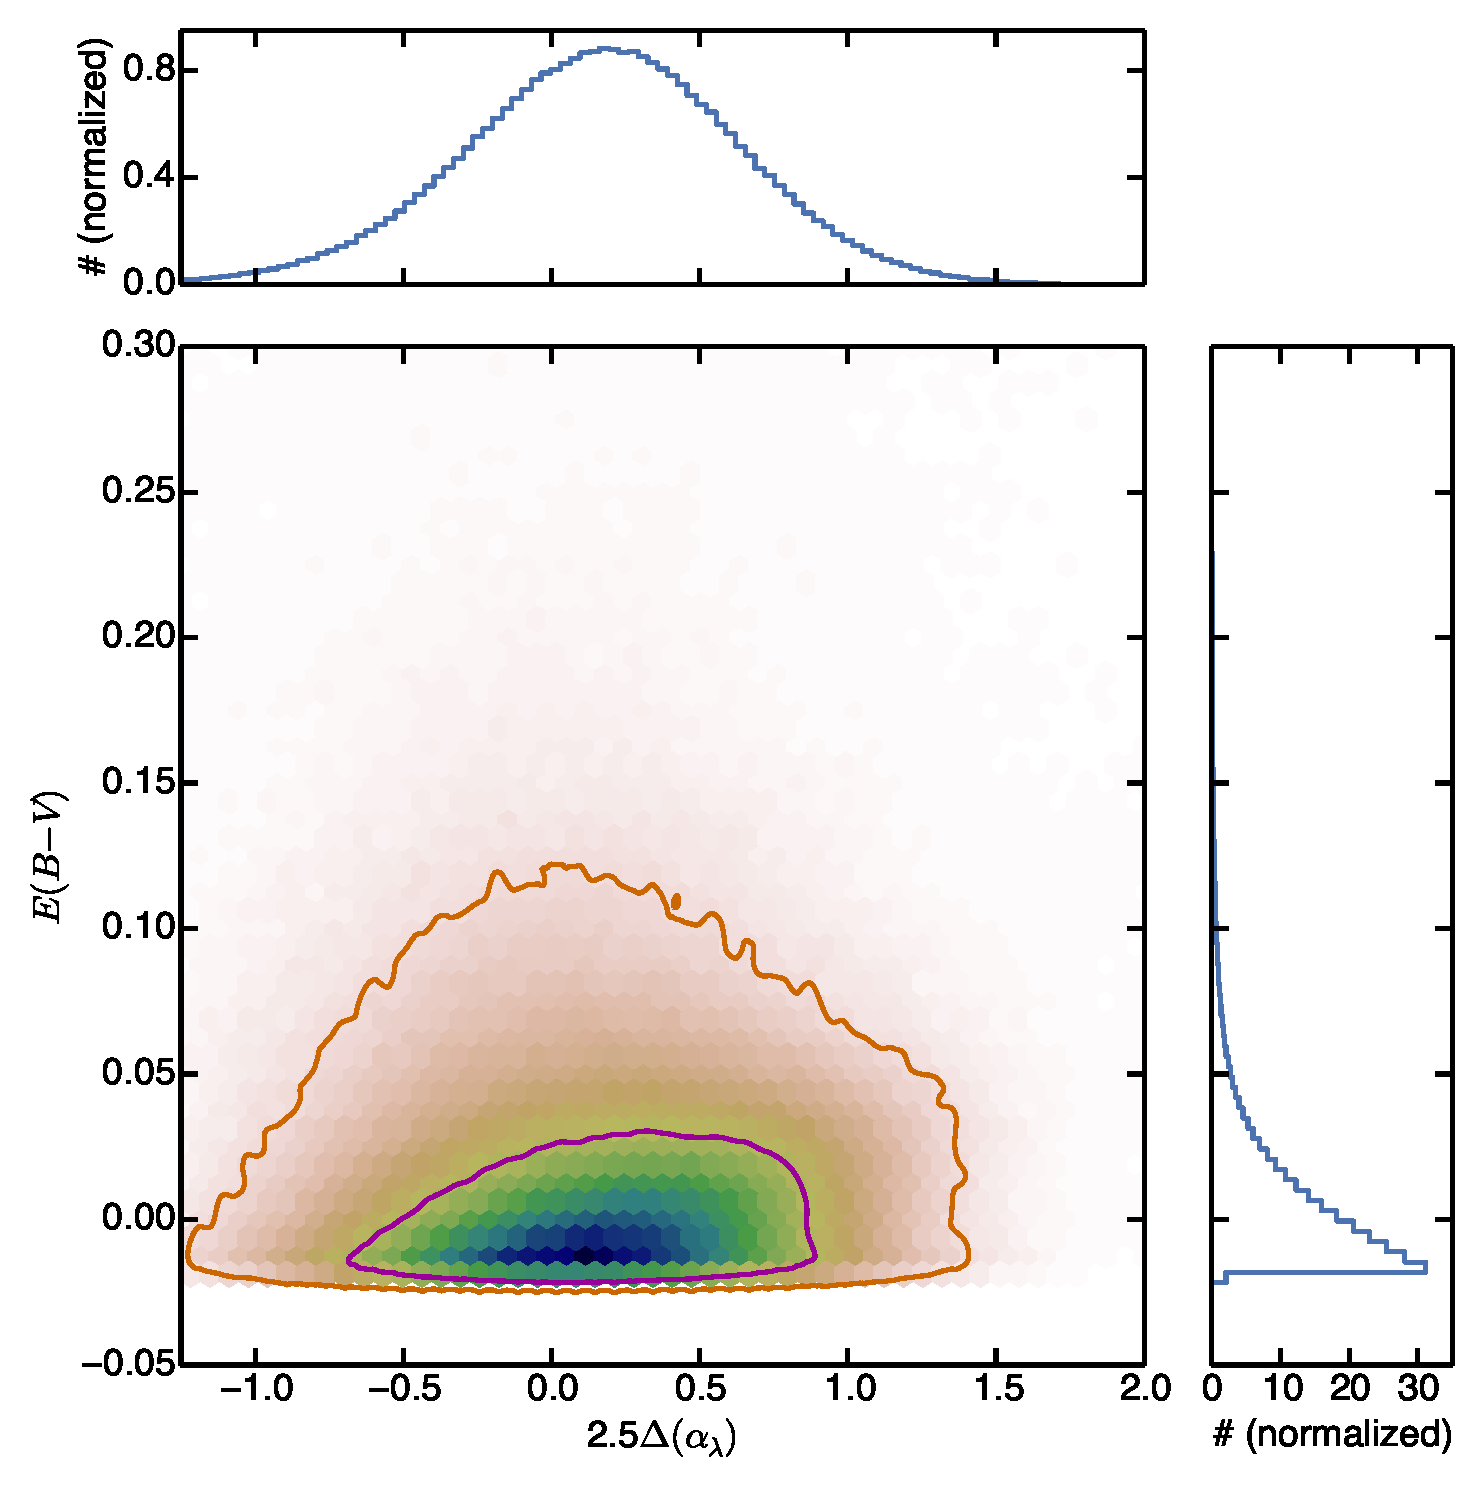
\includegraphics[width=3.1in]{images/Dust/f10a} & 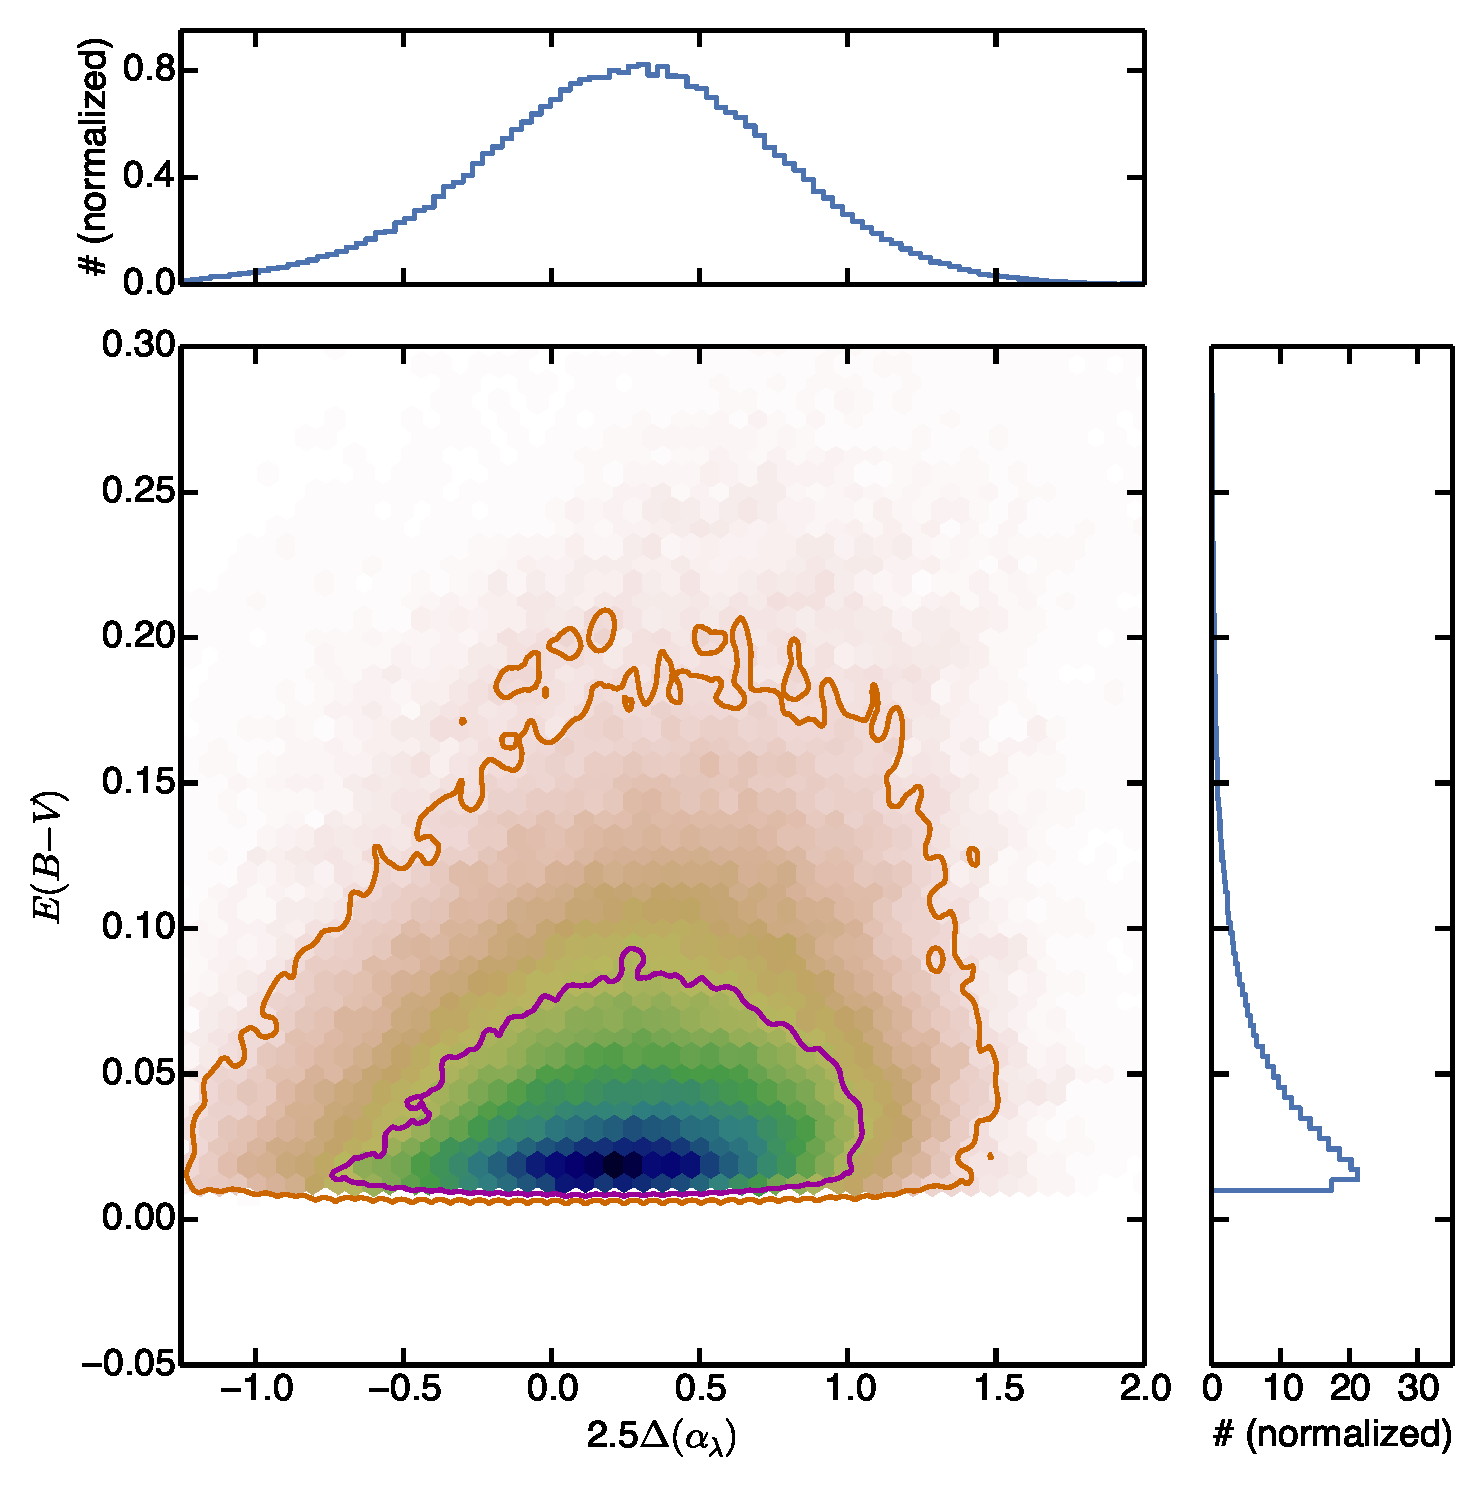
\includegraphics[width=3.1in]{images/Dust/f10b} \\
\end{tabular}
\caption[Joint probability distribution of 2.5$\dal$ and $\ebv$]{\label{fig:indv_fits_SMC} Joint probability distribution of 2.5$\dal$ and $\ebv$ values for non-BAL ({\em left}) and BAL ({\em right}) quasars for the SMC reddening law. The 1$\sigma$ (2$\sigma$) contours are shown in purple (orange) and the fully marginalized distributions for each variable are shown as histograms.  The zero point on the x-axis represents the modal quasar that has $\alpha_{\lambda} =-1.72$ ($\alpha_{\nu}=-0.28$) and positive 2.5$\dal$ values are bluer.  The negative $\ebv$ values on the left argue that the mean non-BAL quasar is not dust reddened (and is $\sim$0.07 bluer in $\alpha_{\lambda}$ than we have assumed).  The positive $\ebv$ values on the right argue that, in contrast to non-BALs, BALs all have dust and are intrinsically bluer than the non-BALs by virtue of the centroid of the blue region. Moreover, at a given $\ebv$, the most probable value for 2.5$\dal$ is larger, suggesting that more heavily reddened BAL quasars are actually intrinsically bluer.}
\end{center}
\end{figure*}

Figures~\ref{fig:indv_fits_SMC} and \ref{fig:indv_fits_L14} show the marginalized joint probability distributions for 2.5$\dal$ and $\ebv$ for each of our samples, i.e. the (2D) probability distribution for each {\em individual} quasar summed together and projected onto the 2.5$\dal$--$\ebv$ plane.  The top and side panels of each plot show the fully marginalized probability distributions for 2.5$\dal$ and $\ebv$ respectively; these distributions are the ones described by the population parameters in Table~\ref{tab:hyp_fit_table}.  The modal quasar ($\alpha_{\lambda} =-1.72$, $\alpha_{\nu}=-0.28$) represents the zero point of the x-axis and positive values of $\dal$ indicate quasars that are bluer than the mode.  

In Figure~\ref{fig:indv_fits_SMC} we show the results for fitting the SMC reddening law.  As was learned from the population parameters, we see that both the non-BAL and BAL samples are (on average) $\sim$0.07 bluer in $\alpha_{\lambda}$ than the modal quasar and the BAL sample shows more dust reddening.  The marginalized distributions for $\ebv$ argue that 2.5\% (13\%) of the non-BAL (BAL) quasars are consistent with $\ebv>0.1$ and 0.1\% (1.3\%) are consistent with $\ebv>0.2$.
Moreover, at a given $\ebv$ value, the BAL quasars are more likely to be bluer, suggesting that more heavily reddened BAL quasars are actually intrinsically bluer.  This trend is not seen in the non-BAL sample.  In both plots we see a lack of quasars that are intrinsically red and heavily dust reddened.  This deficit could be caused by an observational bias, i.e. quasars in this region have colors that are missed by the selection algorithm.  If this is not the case, then this might suggest that the heaviest levels of extinction are associated with the quasar itself rather than the host galaxy, otherwise there would be no link between the intrinsic color and the reddening (unless there is also a link between the host galaxy and the intrinsic quasar color).

In Figure~\ref{fig:indv_fits_L14} we see qualitatively the same trends for the L14-QSO reddening law as we did for the SMC law, the biggest differences being the scaling of the y-axis and a shift in the $\dal$ to smaller values. Here the marginalized distributions for $\ebv$ argue that 0.2\% (1.7\%) of the non-BAL (BAL) quasars are consistent with $\ebv>0.1$ and 0.002\% (0.022\%) are consistent with $\ebv>0.2$.

\begin{figure*}[t]
\begin{center}
%\includegraphics[width=6in]{f8}
\begin{tabular}{cc}
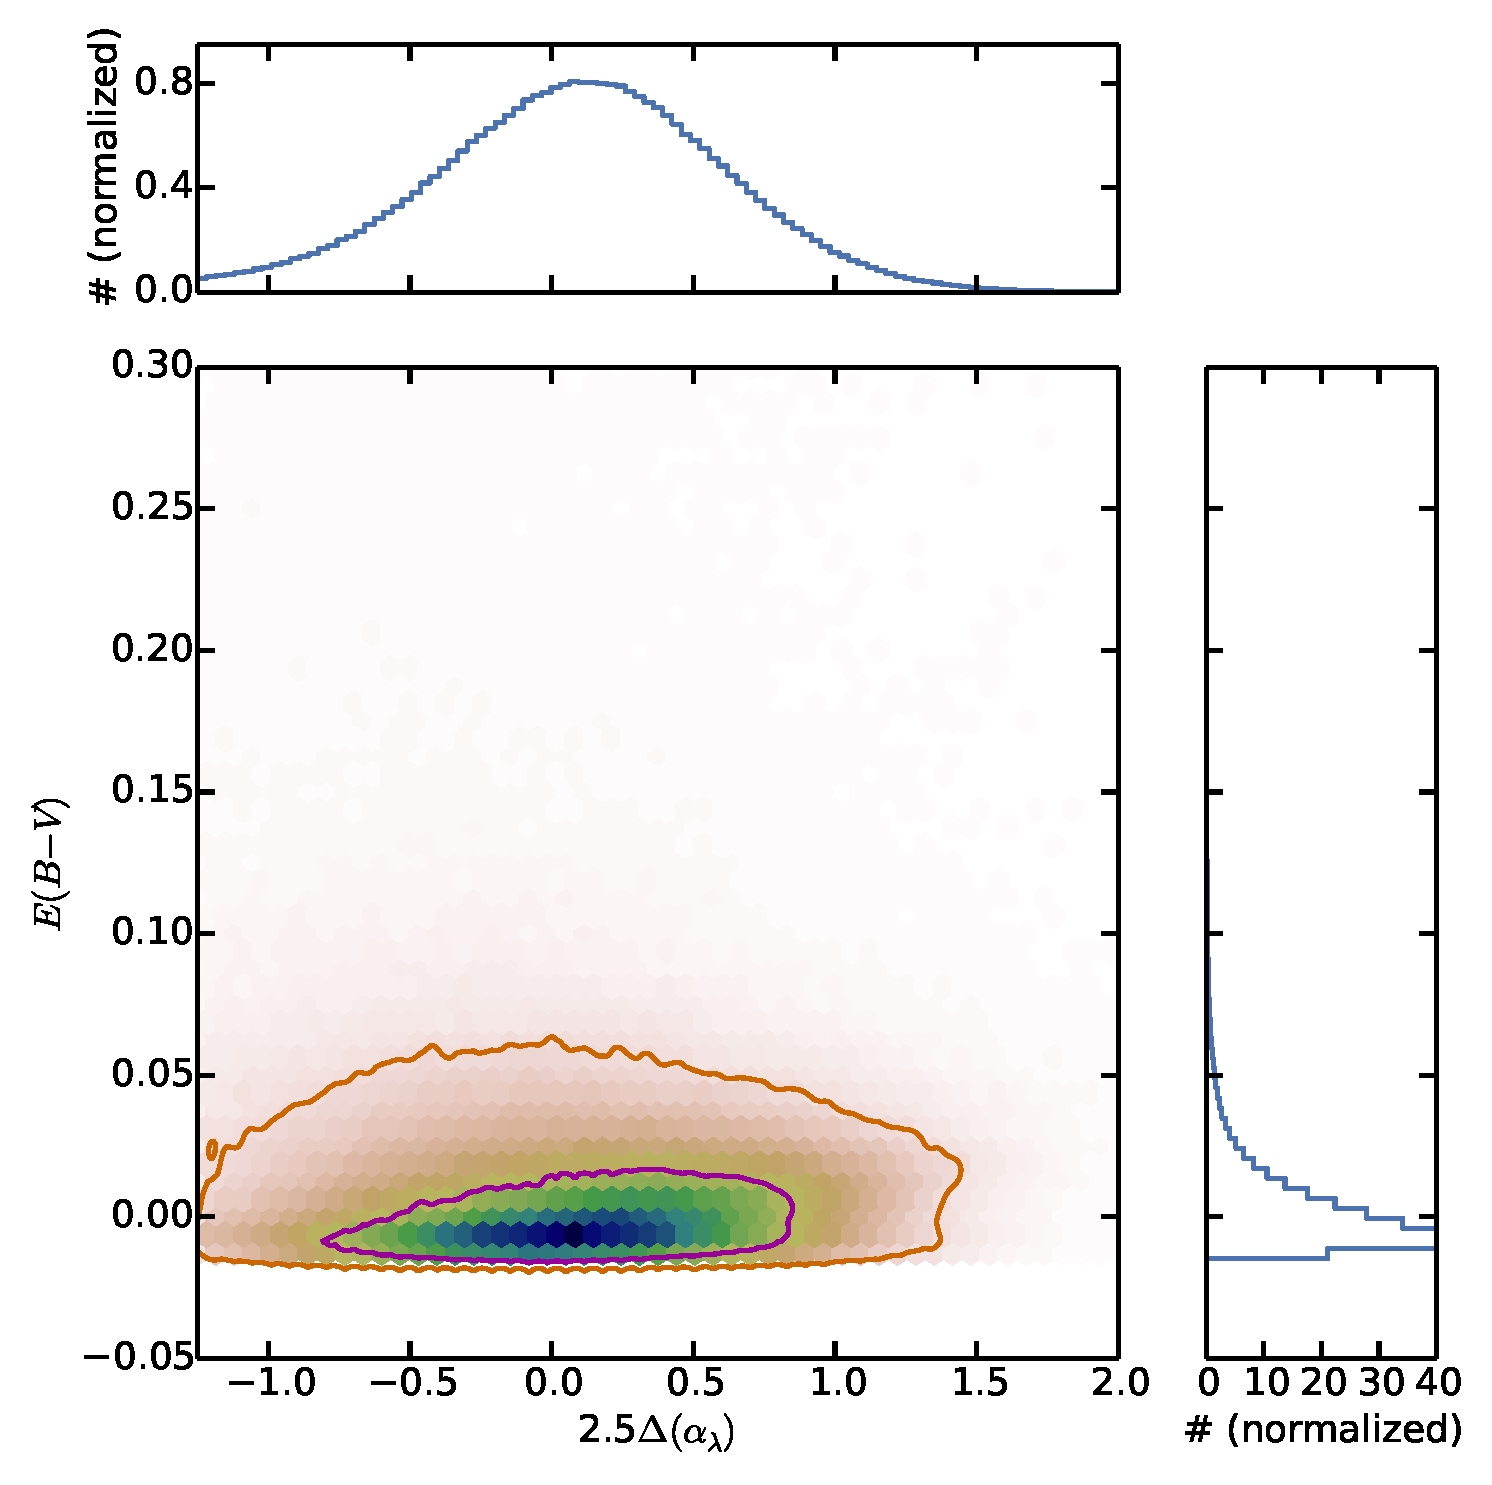
\includegraphics[width=3.1in]{images/Dust/f10c} & 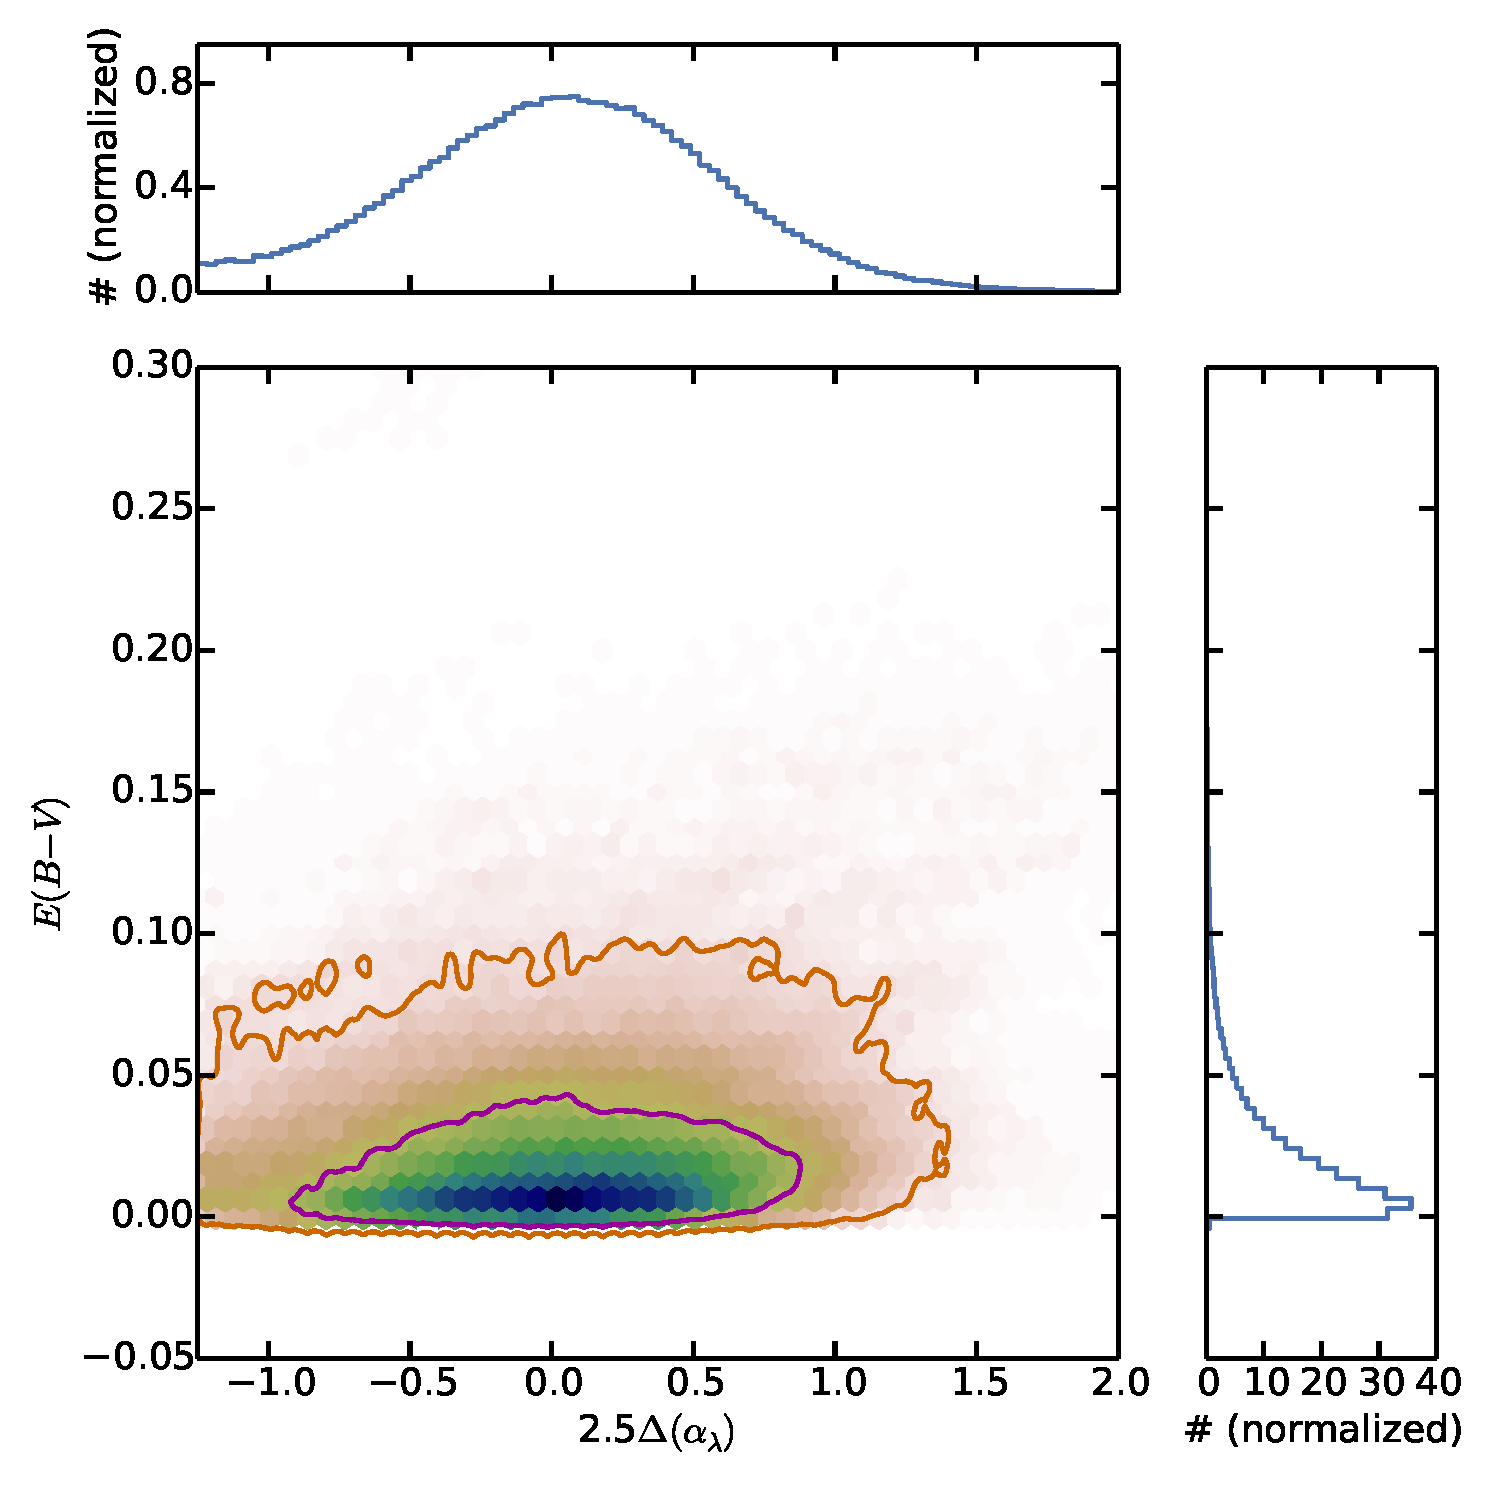
\includegraphics[width=3.1in]{images/Dust/f10d} 
\end{tabular}
\caption[Joint probability distribution of 2.5$\dal$ and $\ebv$]{\label{fig:indv_fits_L14} Same as Figure~\ref{fig:indv_fits_SMC} but using the L14-QSO reddening law.  The general shapes of these distributions are the same but the $\ebv$ values are smaller, as expected for a steeper reddening law.  Again, the BAL quasars show that for a given $\ebv$, the most probable value for 2.5$\dal$ is larger, suggesting that the more heavily reddened BAL quasars are actually intrinsically bluer.}
\end{center}
\end{figure*}

Using this data set, we can also look at the observed BAL fraction as a function of 2.5$\dal$ and $\ebv$.  We have made no attempt to find the intrinsic BAL fraction as was done in \citet{Hewett:2003}, instead, we are looking at how the relative fraction of observed BALs changes as a function of these parameters.  Figure~\ref{fig:bal_frac} shows that the BAL fraction for the SMC and L14-QSO reddening laws.  As with the previous plots, we see that the changes in the BAL fraction are qualitatively similar for both reddening laws: it increases from $\sim0.01$ for red quasars with little dust reddening, up to $\sim0.6$ for blue quasars with heavy dust reddening.  After marginalizing over $\ebv$ we see that the BAL fraction ranges between $\sim0.05$ and $\sim0.2$ and it clearly increases as quasars become bluer.   This trend has only become clear due to our larger data set, and is in comparison to previous studies \citep[e.g. ][]{Tolea:2002,Hewett:2003,Reichard:2003b} that were only able to measure the mean BAL fraction of $\sim20\%$.
%This is in contrast to the constant BAL fraction of $\sim20\%$ seen throughout the literature \citep[e.g. ][]{Tolea:2002,Hewett:2003,Reichard:2003b}.  
As with Figures~\ref{fig:indv_fits_SMC} and \ref{fig:indv_fits_L14} we have marginalized over the probability distributions for each individual quasar, meaning the trend seen here is expected to be real (up to any observational biases) and not an artifact of our model. 

\begin{figure*}[t]
\begin{center}
\begin{tabular}{cc}
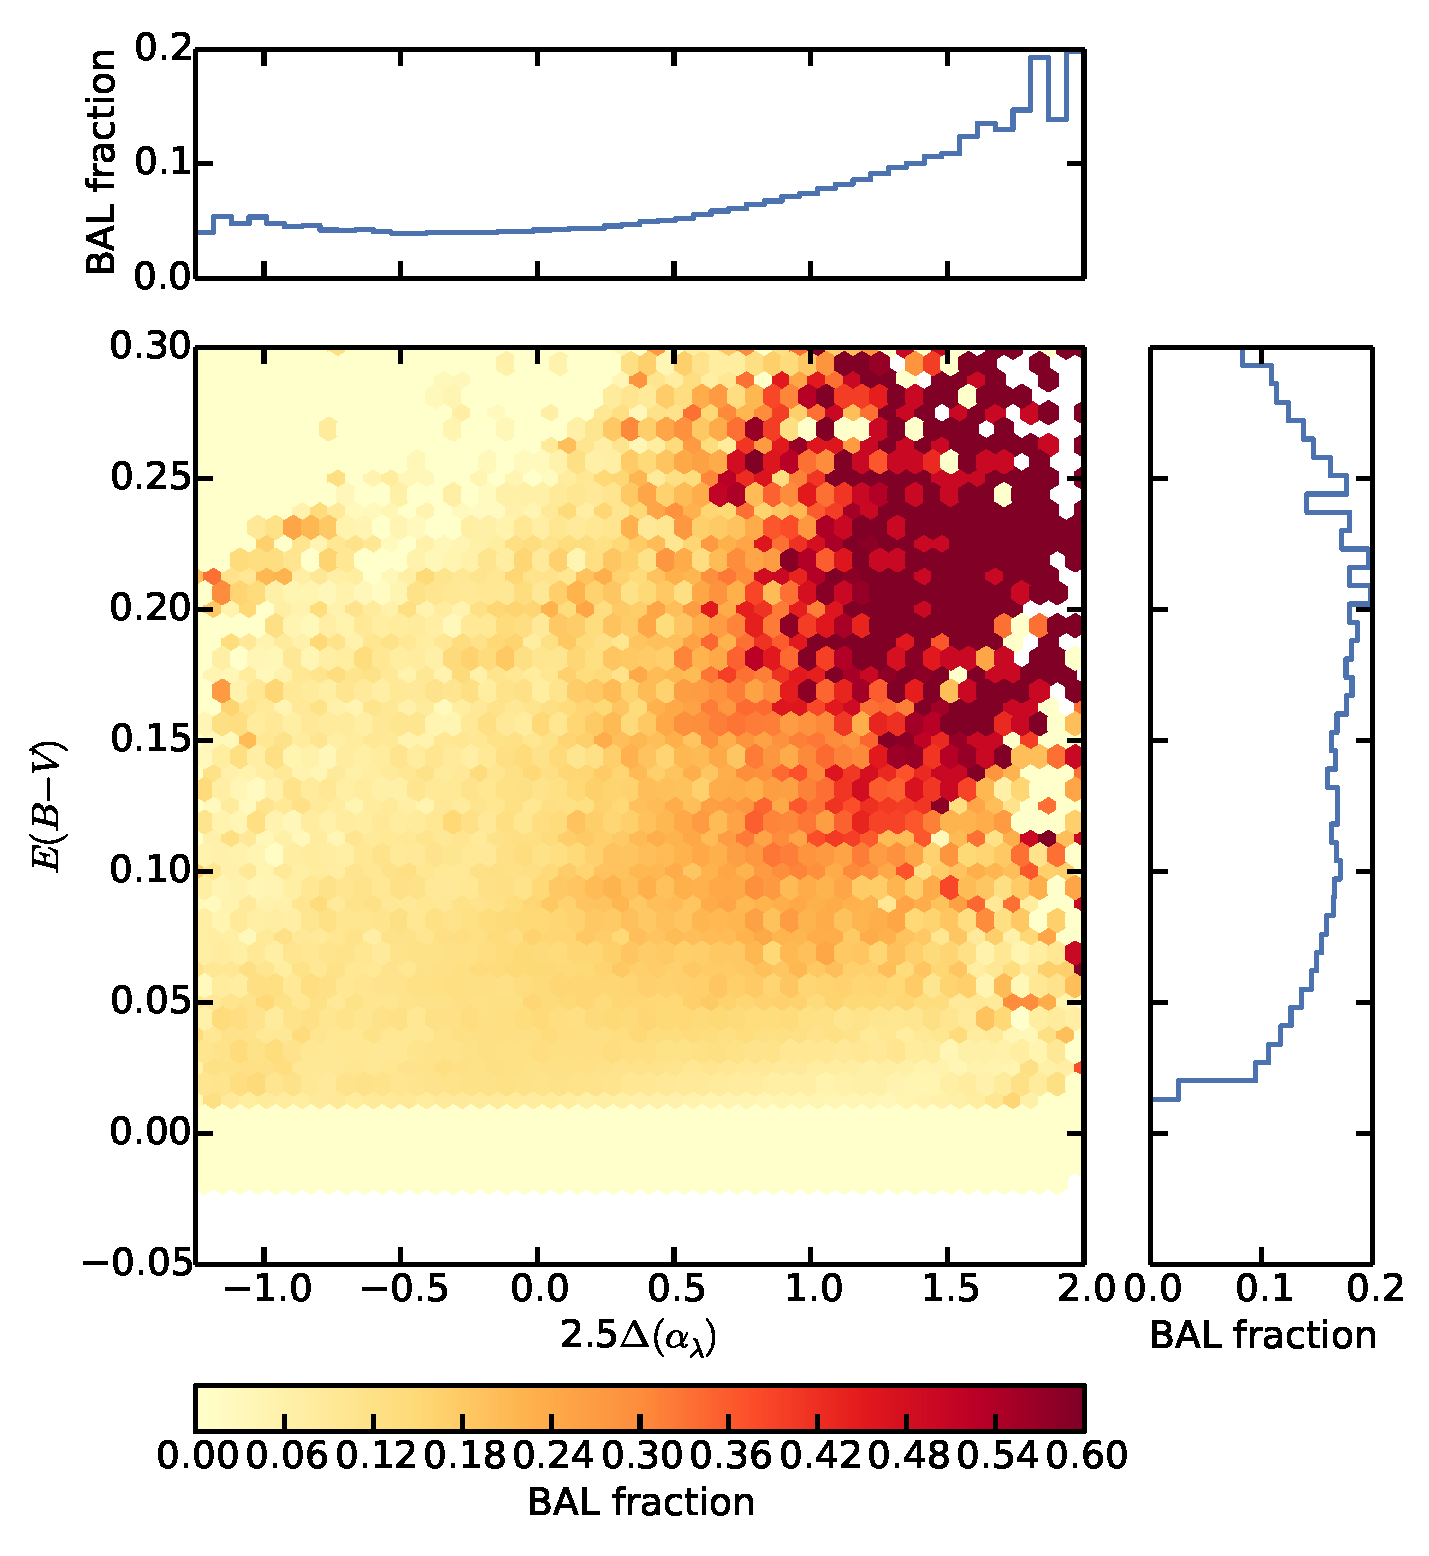
\includegraphics[width=3.1in]{images/Dust/f11a} & 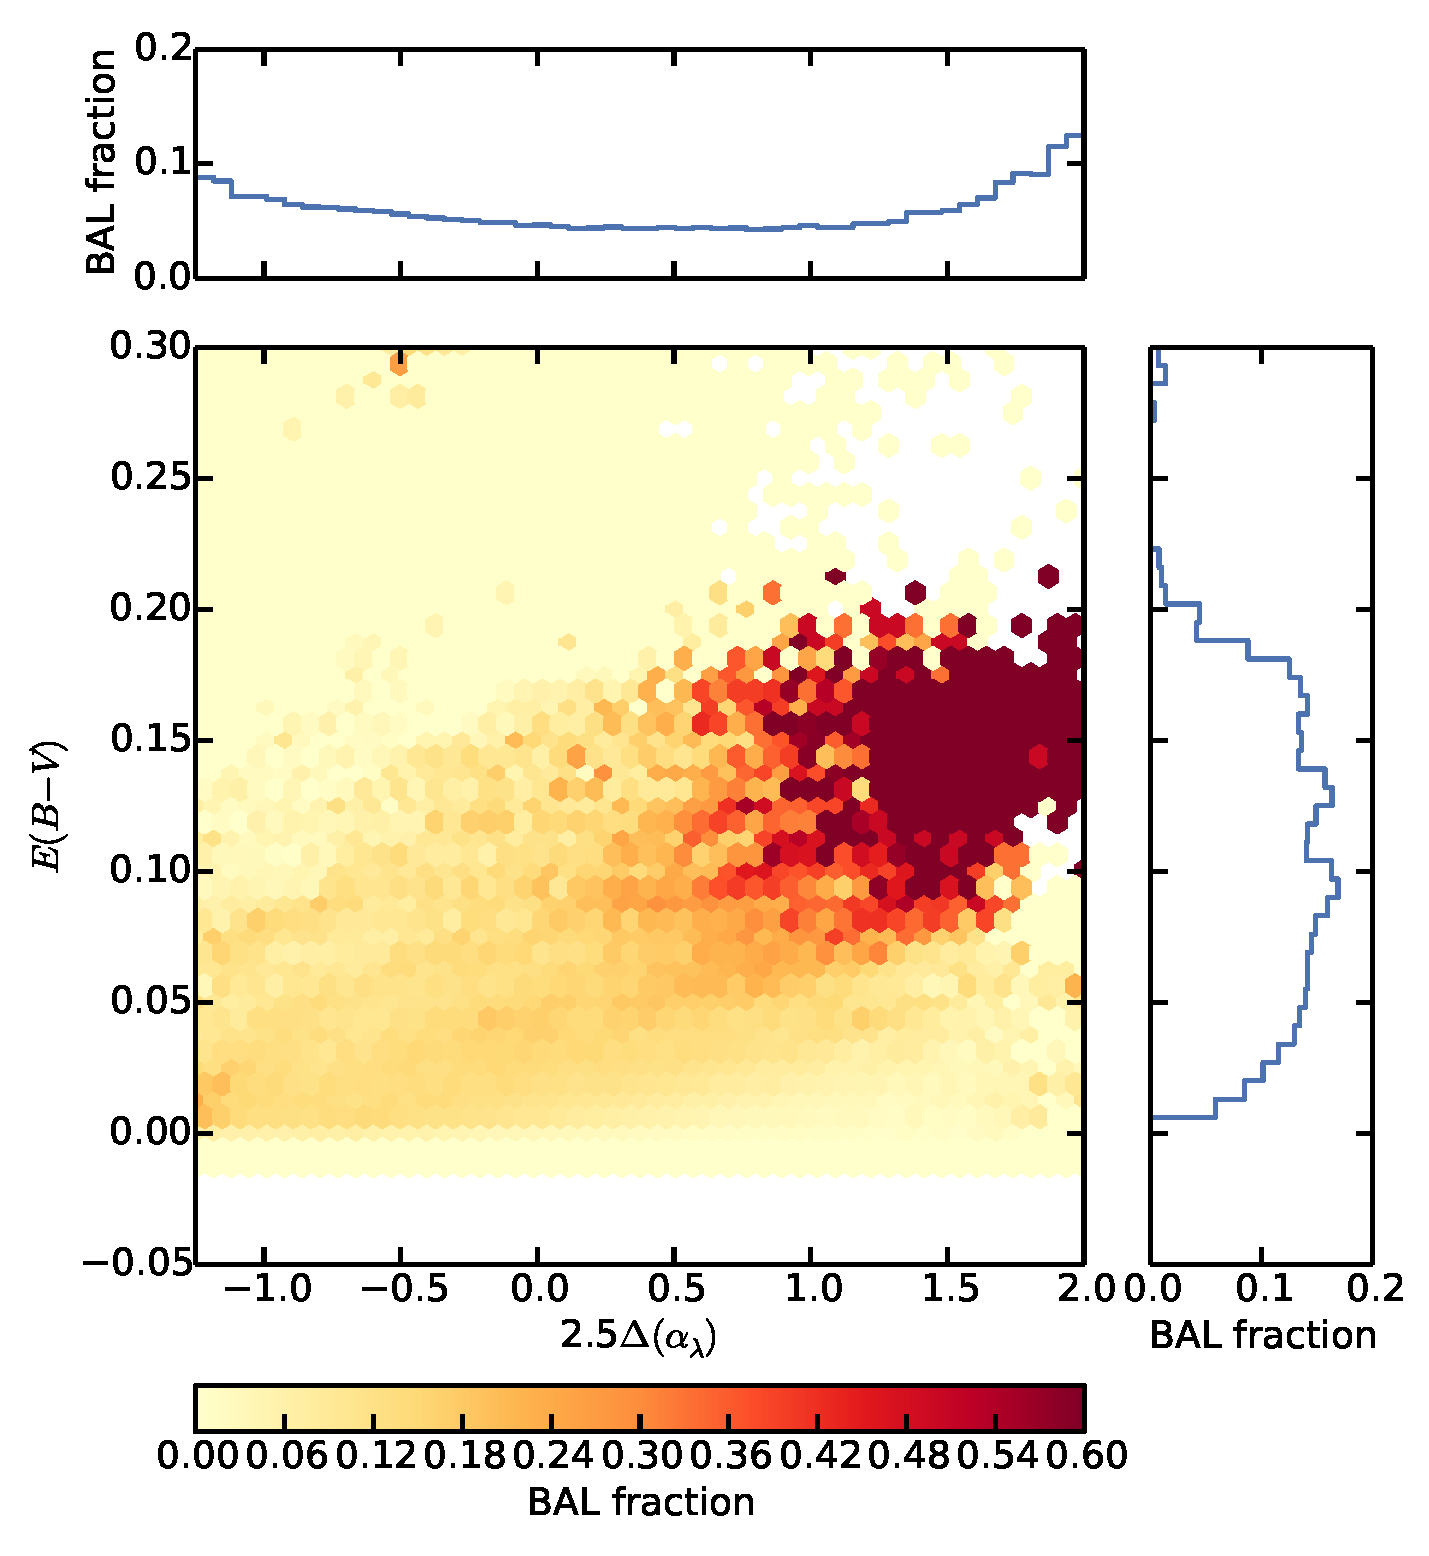
\includegraphics[width=3.1in]{images/Dust/f11b} 
\end{tabular}
\caption[BAL fraction]{\label{fig:bal_frac} The fraction of BAL quasars as a function of 2.5$\dal$ and $\ebv$ for the SMC reddening law ({\em left}) and the L14-QSO reddening law ({\em right}).  The fully marginalized BAL fractions are shown in the histograms.  We can see the BAL fraction goes from $\sim0.01$ to $\sim0.6$ as the intrinsic color becomes bluer and the amount of dust increases.  Although the BAL fraction reaches $\sim0.6$ in the 2D parameters space, it does not exceed $\sim0.2$ after marginalizing over $\ebv$.}
\end{center}
\end{figure*}

This analysis suggests that the parent populations for BALs and non-BALs are slightly different (BALs being intrinsically bluer, on average).  However, we need to be careful that selection effects are not involved.  For example, \citet{Reichard:2003b} discussed how the probability of SDSS finding a BAL changes with redshift.

%Although we find the parent distributions for our BAL and non-BAL samples to be different, it can be argued  that the parent distributions are not necessarily intrinsically different. The observed difference could be caused by a selection effect. In color-color space intrinsically blue quasars overlap the stellar locus between the redshifts of 2.7 and 3 [are these numbers right], making them difficult to identify.  If these quasars have a sufficient amount of dust [should figure out how much] they will be shifted out of the stellar locus making them easier to identify.  Since BAL quasars are more heavily reddened than their non-BAL counterparts, we are more likely to identify intrinsically blue BALs than intrinsically blue non-BALs in this redshift range.  Alternatively the parent distributions could be intrinsically different and bluer quasars have a large probability of have BALs (e.g. bluer quasars are more likely to have a disk wind) than redder ones.

\subsection{What Reddening Law Fits Better?}\label{sec:DIC}

Given that we used two different reddening laws to fit our data, it is natural to ask: what reddening laws fits the data better?  To answer this question we use the deviance information criterion (DIC).  The DIC is a generalization of the Bayesian information criterion (BIC) such that it can be directly applied to the output of an MCMC fit, and can be used to directly compare multiple models fit to the same data.  The DIC is made up to two terms, one that is related to the likelihood of the model explaining the data (similar to $\chi^2$), and a penalty term based on the complexity of the model (i.e. the effective degrees of freedom after taking into account the covariances between the fitted variables).  

Models that have smaller DIC values fit the data better than models with higher DIC value, and the size of this difference gives a measure of how much better the fit is.  When the difference is less then 2 both models fit the data well, when it is between 2 and 6 there is positive evidence for the lower model fitting better, and when it is greater then 6 there is strong evidence.  We have calculated the DIC for each individual quasar to see what model fits better, these values are included in Table~\ref{tab:ind_fits}.  Table~\ref{tab:model_compare} summarizes the comparison of the two models.  Overall we find the SMC reddening law does a better job fitting our data, and to the end of applying the best correction in the mean sense, it will be used exclusively for the remainder of this thesis.  However, we do find that up to 4\% (11\%) of non-BAL (BAL) quasars show signs of contributions from multiple scattering, and for future work it may be interesting to consider this subset to see how they differ from the main sample.

%for future work it may be interesting to consider the subset of quasars that are better fit by the multiple-scattering law, and see how they differ from the main sample.

%[However, for future work it may be important to consider that a multiple-scattering law better fits a fraction of the data (and is most consistent with the dashed line in Figure 4.4 -- what do you make of that?]

\begin{deluxetable}{lrrrrr}
\tablewidth{0pt}

\tablecaption{\label{tab:model_compare} Reddening Law Comparison}
\tablehead{
\colhead{} & \multicolumn{2}{c}{non-BAL} & \colhead{} & \multicolumn{2}{c}{BAL} \\
\cline{2-3} \cline{5-6}\\
\colhead{Evidence} & \colhead{Number} & \colhead{Fraction} & \colhead{} & \colhead{Number} & \colhead{Fraction}
}
\startdata
SMC: strong            & 23443 & 68.5\% & & 1131 & 64.9\% \\
SMC: positive          & 9291 & 27.1\% & & 414 & 23.7\% \\
Both                          & 1470 & 4.3\% & & 192 & 11.0\% \\
L14-QSO: positive & 16 & 0.05\% & & 5 & 0.3\% \\
L14-QSO: strong    & 6 & 0.01\% & & 2 & 0.1\%
\enddata
\end{deluxetable}

\section{Composite Spectra} \label{sec:spectra}

\citet{Hopkins:2004} discuss composite spectra as functions of the ($c_1$,$c_2$) parameter space.  Here we construct composite spectra based on the more physical parameter space of 2.5$\dal$ and $\ebv$ from the previous section.  Our composites are constructed in the same way as the \citet{Vanden-Berk:2001} quasar composite, using similar code. In brief, the quasars are sorted by redshift, shifted to their rest frames, re-sampled onto a common 1\AA\ grid, and normalized by the overlap with the current composite.  To preserve the continuum shape in the composite we chose to use a weighted geometric mean to combine the spectra \citep{Vanden-Berk:2001,Reichard:2003b}.

The spectra were split into ten equally spaced bins in both 2.5$\dal$ and $\ebv$. The MCMC sampler from \S\ref{sec:mcmc} produced full probability distributions for each quasar in this parameter space, allowing us to find the probability for each quasar belonging to any given bin.
This probability was used as the weight when calculating the geometric mean in each bin. To prevent quasars with high variance (i.e. spread across many bins) from contaminating the sample, only quasars with a probability of being in a bin greater than 10\% were used. After this cut, composites were made for any bin with more than ten quasars.

\subsection{Red vs. Reddened: Spectra}
Figures~\ref{fig:spec} and~\ref{fig:bal_spec} show the resulting composites for the non-BAL and BAL samples respectively. Each panel in these figures corresponds to a single 2.5$\dal$ bin (the 10th bin for each sample had too few quasars to stack) and each color corresponds to a single $\ebv$ bin. The black dashed lines show the typical intrinsic powerlaw in each bin (red to blue going from the top left to bottom right) with the red dashed lines showing the global modal powerlaw, $\alpha_{\lambda}=-1.72$ ($\alpha_{\nu}=-0.28$), for comparison.  The color dashed lines show the typical powerlaw for each bin reddened by the $\ebv$ values corresponding to each color.  In most cases we see that the color dashed lines are in agreement with the stacked spectra in each bin, indicating that the 2.5$\dal$ and $\ebv$ values found in the previous section are accurate.  The notable exceptions are the most reddened bin for almost all the 2.5$\dal$ bins, these spectra tend to show more curvature than would be expected from the fits to their photometry suggesting, that, if anything, those quasars are better fit by a steeper reddening law (such as multiple-scattering). 

\begin{figure*}
\begin{center}
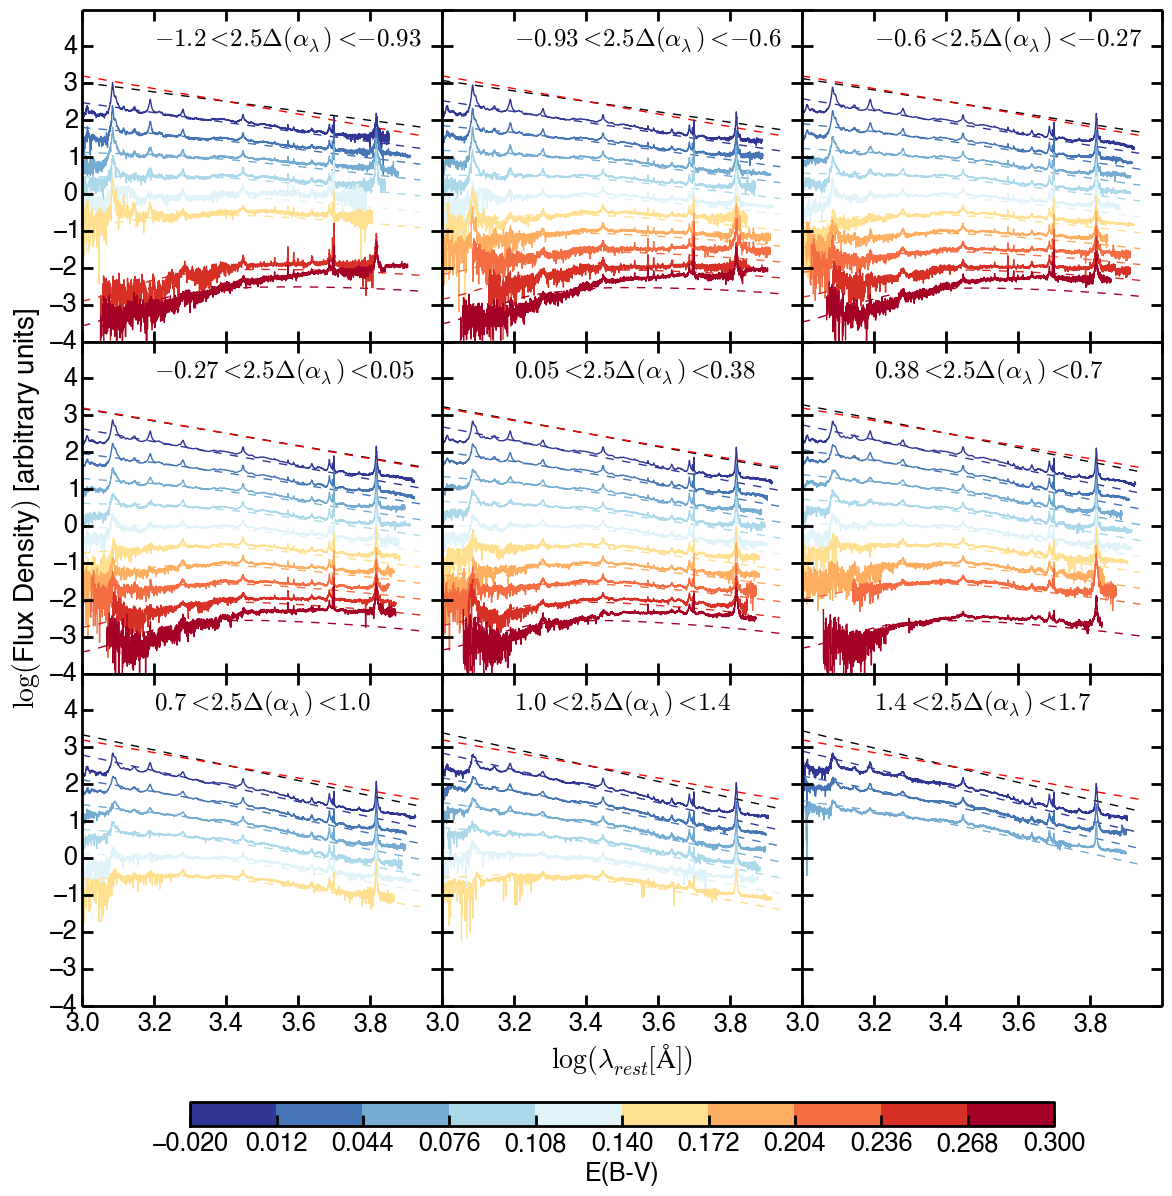
\includegraphics[width=6.25in]{images/Dust/f12}
\caption[Composite spectra for non-BAL quasars]{\label{fig:spec} Composite spectra for non-BAL quasars (solid lines) for nine evenly spaced bins along 2.5$\dal$ (subplots going intrinsically red to blue from the top left to the bottom right) and for ten evenly spaced bins along $\ebv$ (various colors) based on the fits to the SMC reddening law.  The black dashed line in each panel indicates the typical powerlaw for each quasar in that 2.5$\dal$ bin and the red dashed line shows the observed modal powerlaw ($\dal=0$) for comparison.  The colored dashed lines show the typical powerlaw reddened by the $\ebv$ value corresponding to each color. The middle-left panel shows objects with spectral indices most similar to the modal powerlaw.  The objects best fit by an intrinsically bluer spectrum demonstrate that such objects exist, but the bluest spectra that are best fit without any dust are not perfect fits.  This could be a sign of mis-fitting, or may be an indication of the spectral turn-over within the fitting region (which is expected from \citet{Shang:2005}).  Each composite spectrum is largely in agreement with the bin values found from fitting the photometry.}
\end{center}
\end{figure*}

We also see slight deviations in the bluest bin for the least reddened spectra.  One potential cause for this deviation is if the underlying continuum between 1\,$\mu$m and 1216\,\AA\ is not well described by a powerlaw.  The continuum emission from a quasar is thought to come from a modified blackbody \citep{Shakura:1976} that has been seen to turn over at wavelengths of about $\sim$1000--1300\,\AA\ \citep{Shang:2005}. If this turn over happens within the fitting range of our model, these quasars will be erroneously fit with large $\ebv$ values and have curvatures that are different than that caused by an SMC law. %\citet{Krawczyk:2013} found that more luminous quasars tended to turn over at longer wavelengths than less luminous quasars, if these objects are also intrinsically bluer, 

\begin{figure*}
\begin{center}
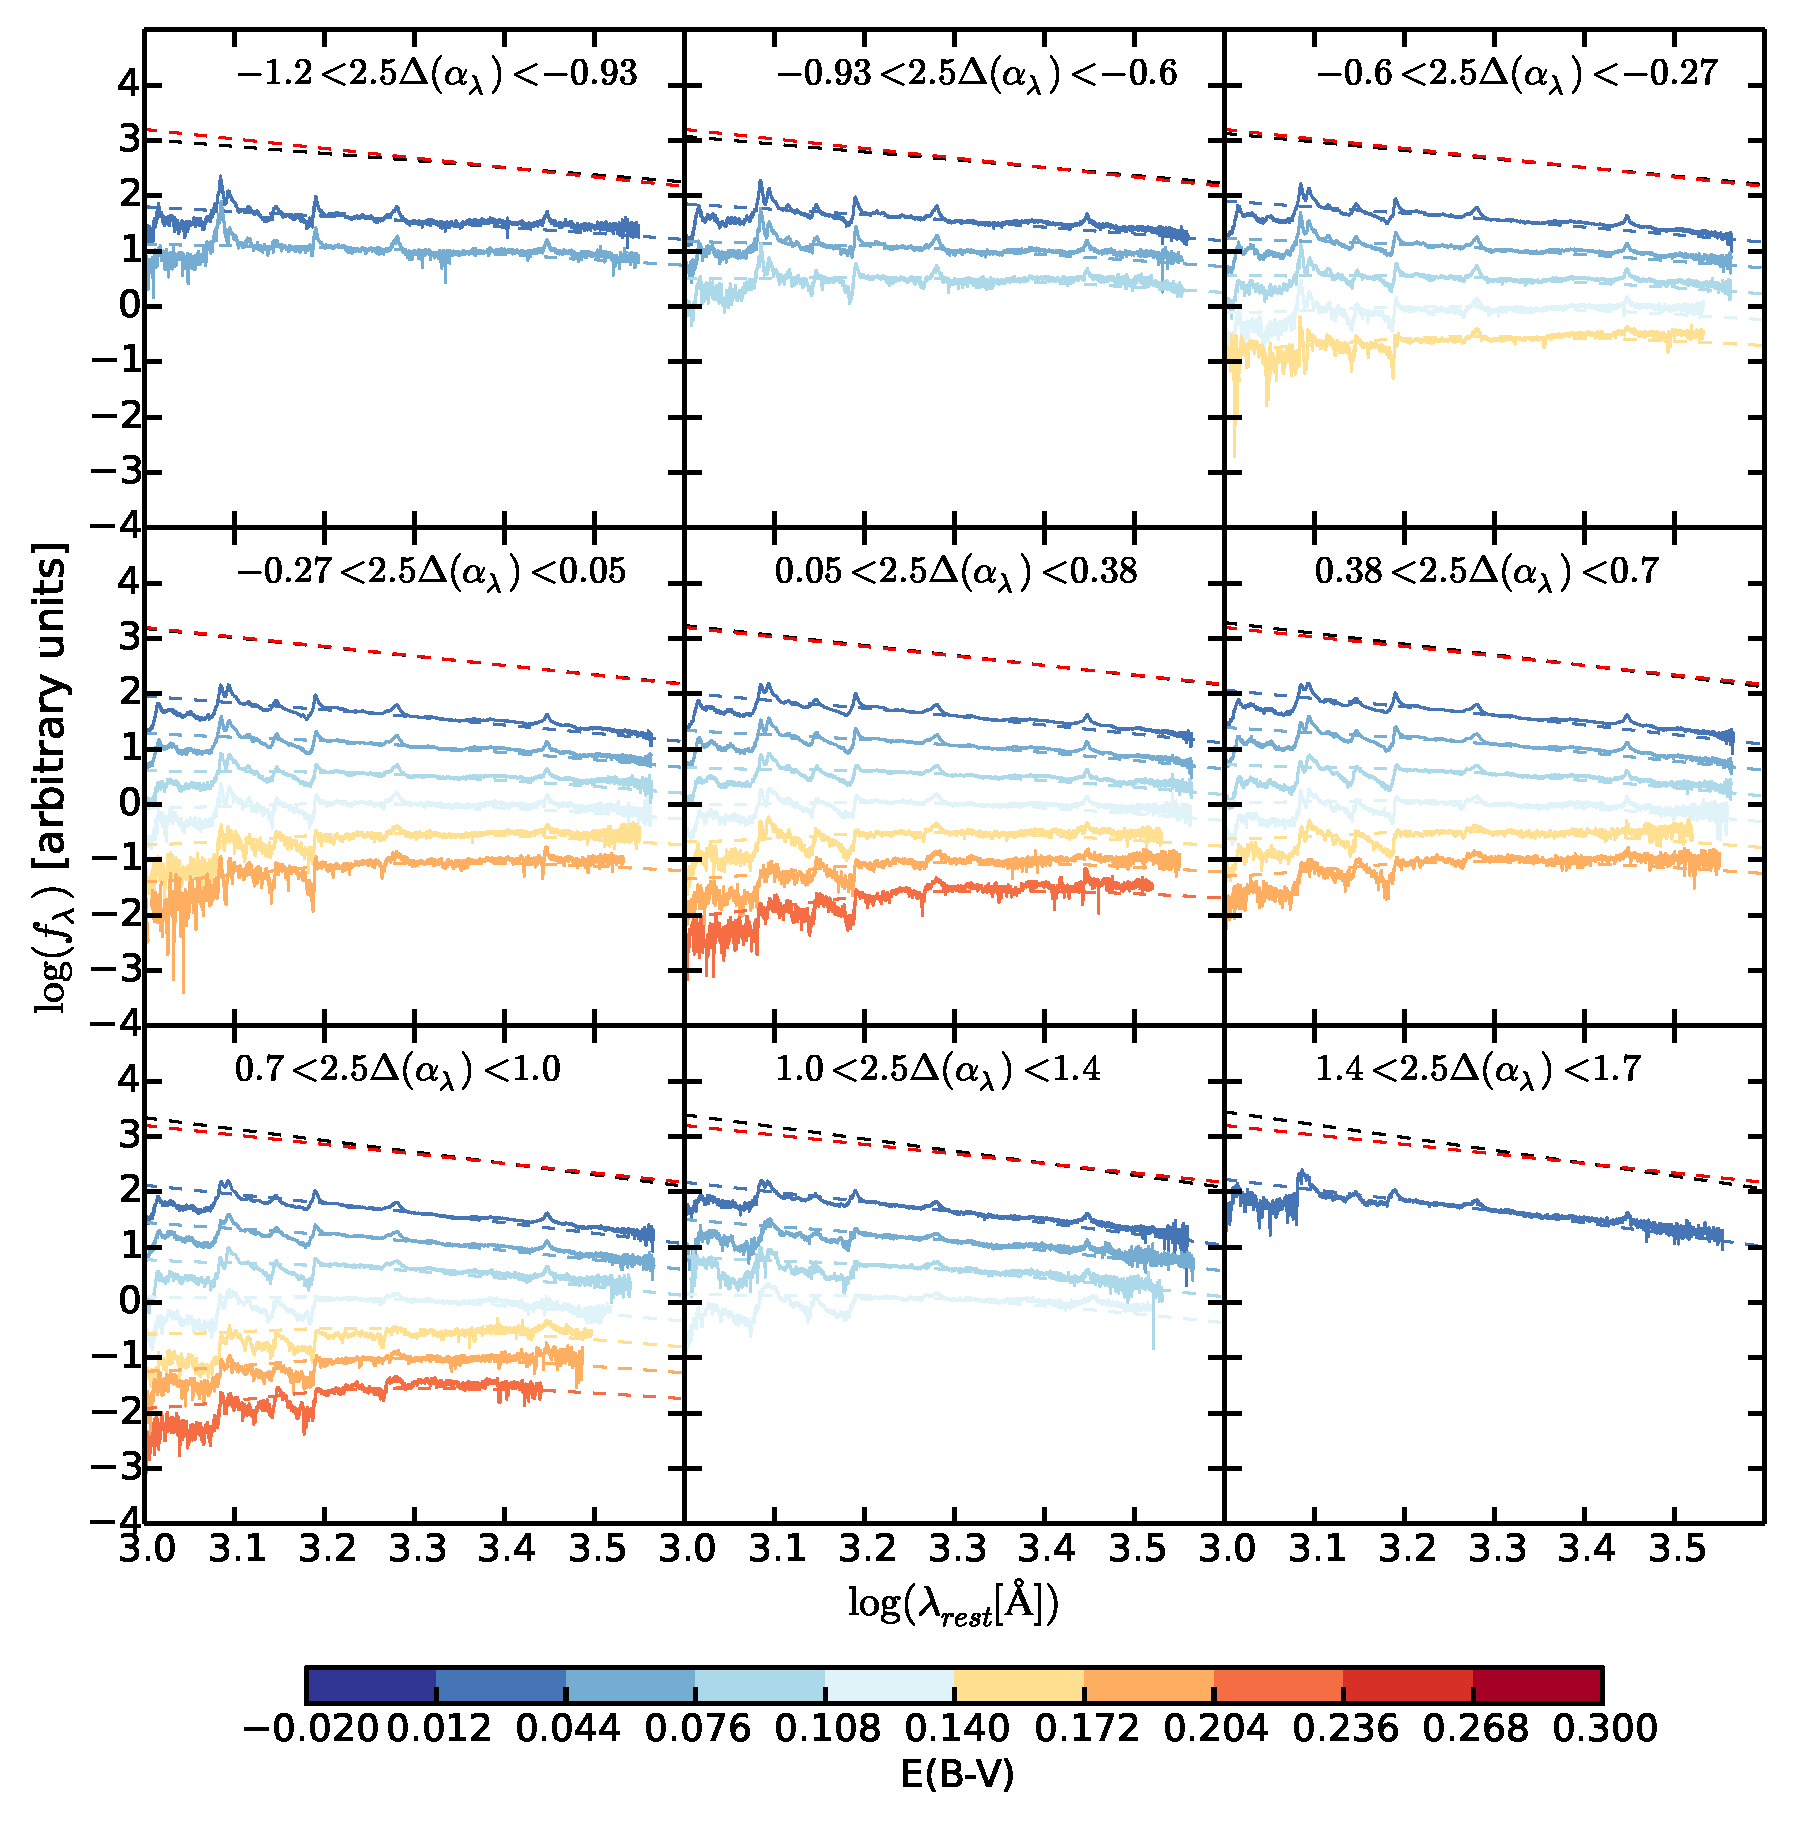
\includegraphics[width=6.25in]{images/Dust/f13}
\caption[Composite spectra for BAL quasars]{\label{fig:bal_spec} 
%Composite spectra for BAL quasars (solid lines) for ten evenly spaced bins along $\ebv$ (various colors) and nine evenly spaced bins along 2.5$\dal$ (subplots).  The black dashed line in each panel indicates the typical powerlaw for each quasar in that 2.5$\dal$ bin and the red dashed line shows the observed modal powerlaw ($\dal=0$) for comparison.  The colored dashed lines show the typical powerlaw reddened by the $\ebv$ value corresponding to each color. The middle-left panel shows objects with spectral indices most similar to the modal powerlaw.  
Same as Figure~\ref{fig:spec} but for the BAL sample.
Within each panel there is an increase in the depth of the \ion{C}{4} absorption trough ($\log{(\lambda)}\sim3.2$) as the $\ebv$ values increase.  The \ion{C}{4} absorption trough also becomes wider as quasars become bluer (e.g. the trough extends out to the nearby \ion{Si}{4} line for the bluest quasars).
%in the fraction of LoBAL quasars (absorption troughs blueward of \ion{Mg}{2}) as the $\ebv$ values increase. This trend is expected from the orientation-dependent picture presented in \citet{Weymann:1991}. We also see that every spectrum is consistent with at least some amount of dust reddening ($\ebv>0.012$). 
Each composite spectrum is largely in agreement with the bin values found from fitting the photometry.}
\end{center}
\end{figure*}

For the BAL quasars in Figure~\ref{fig:bal_spec} we see a trend in \ion{C}{4} absorption ($\log{(\lambda)}\sim3.2$) with 2.5$\dal$ and $\ebv$.  At a given 2.5$\dal$ value the absorption trough for \ion{C}{4} deepens as $\ebv$ increases.  When holding $\ebv$ at a fixed value, the absorption trough becomes wider (and extends to higher velocities) 
for bluer colors than redder colors.  These trends are consistent with the findings of \citet{Baskin:2013} who found \ion{C}{4} troughs become wider as the strength of \ion{He}{2} decreased, a trend we find also corresponds to the non-BAL quasars being bluer (see \S\ref{sec:indv_lines}).  They also found the depth of the \ion{C}{4} trough increased as $\alpha_{\rm UV1}$ became redder, a quantity they associated with dust reddening.

\subsection{Individual Lines} \label{sec:indv_lines}
\citet{Richards:2003} constructed several composite spectra based on the observed $\dgi$ relative colors. They were able to construct four spectra that had little dust reddening and span different spectral indices.  By comparing these spectra they found several trends in individual spectral lines related to the intrinsic slopes. Our analysis provides a more robust metric for distinguish intrinsically red and dust reddened quasars, allowing us to create a cleaner sample of quasars that are thought to be relatively free of dust. This process is useful as one expects a physical link between the continuum and the (photoionized) gas in the BELR.

In this section we explore the trends in some individual emission lines as a function of the intrinsic spectral index for the non-BAL quasars consistent with little to no reddening (i.e. the lowest $\ebv$ bin).  To prevent being influenced by known trends due to quasar luminosity, we picked sub-samples from each bin such that the distribution of \ltwofive, taken from \citet{Krawczyk:2013}, was the same for every sample. When doing this we excluded the two bluest bins from the analysis seeing as their \ltwofive\ distributions were significantly lower than the other bins\footnote{This lower \ltwofive\ distribution is cased by lower redshift distribution for the bluest quasars (see Figure~\ref{l_z_alpha}).}.  The resulting luminosity distribution for the non-BAL sample had $44.4<\log{(L_{2500\,\AA}{\rm \ [ergs\ s^{-1}]})}<47$ and a median of 45.7, while the BAL sample had $46<\log{(L_{2500\,\AA}{\rm \ [ergs\ s^{-1}]})}<46.7$ and a median of 46.2.

\begin{figure*}[t]
\begin{center}
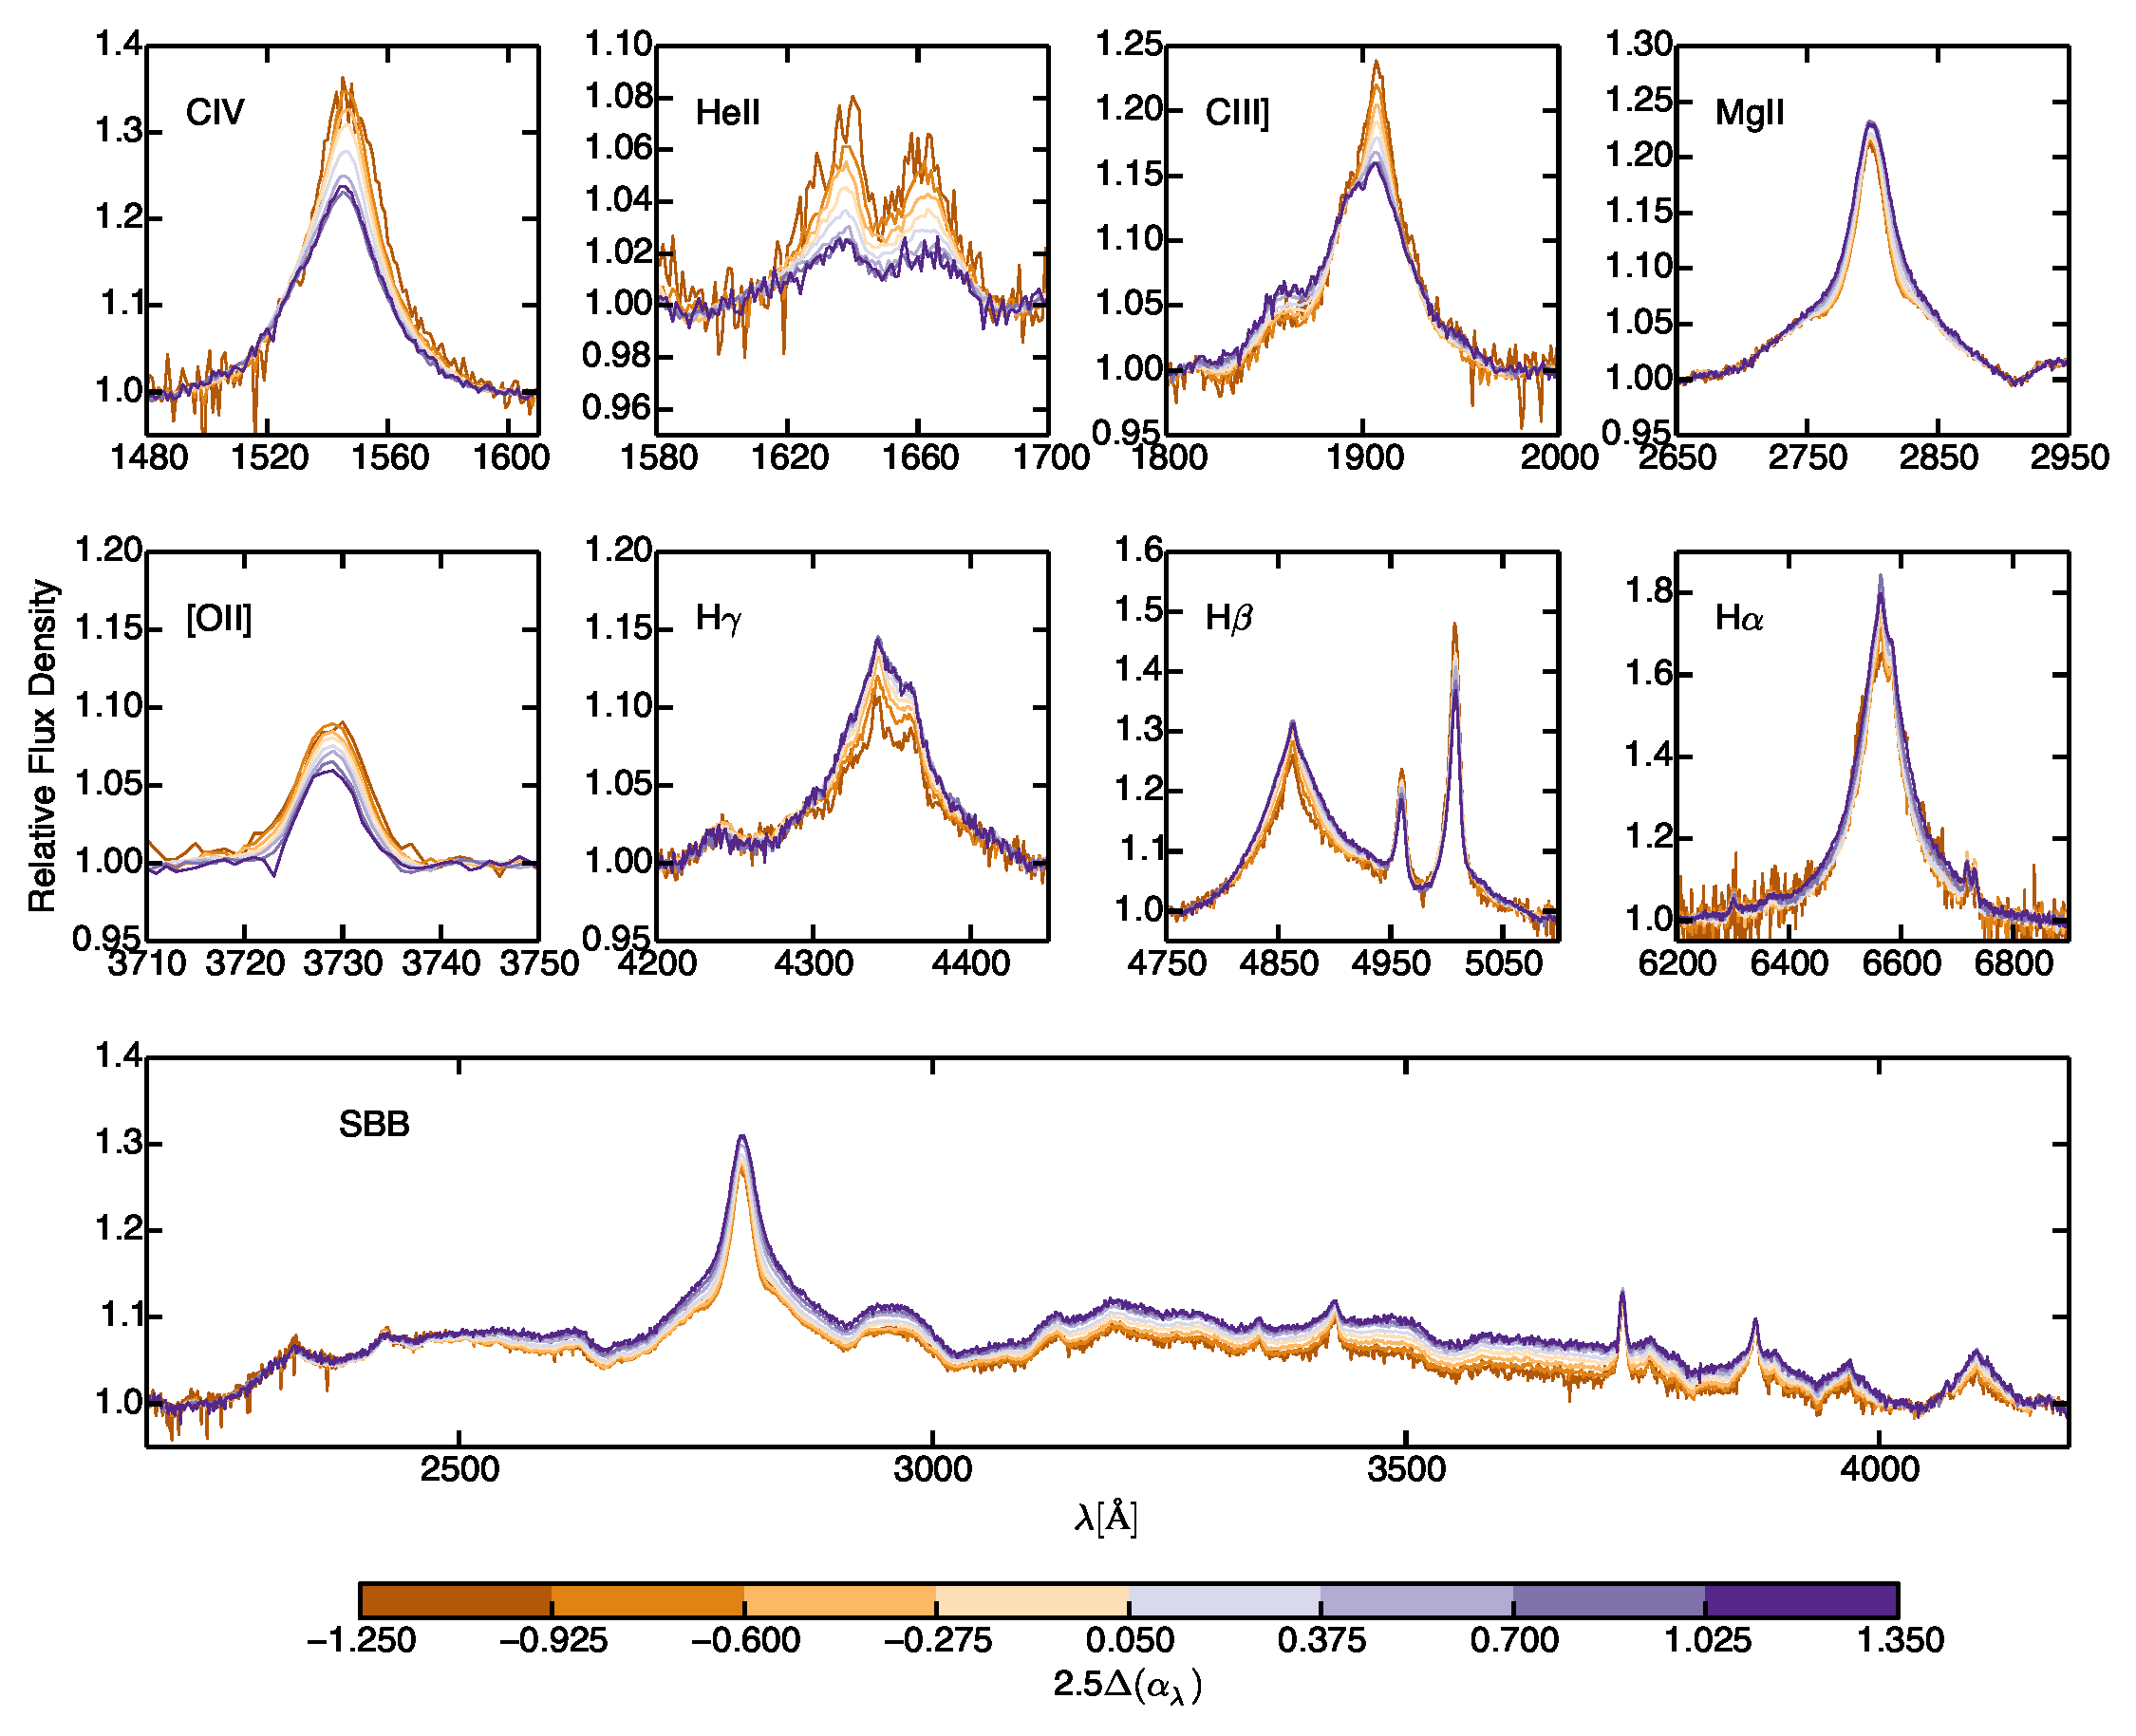
\includegraphics[width=5.95in]{images/Dust/f14}
\caption[Expanded emission-line regions for non-BAL quasars]{\label{fig:ind_spec} Expanded emission-line regions from the lowest $\ebv$ bin from Figure~\ref{fig:spec} ($\ebv<0.012$). ``SBB'' refers to the 3000 \AA\ (or small blue) bump.  The colors represent the 2.5$\dal$ value for each spectrum.  The spectra are normalized such that their continua agree at the edges of the panels.}
\end{center}
\end{figure*}

The major emission line regions are shown in Figure~\ref{fig:ind_spec}. These spectra have been normalized such that they are unity at the edges of each plot. Below we comment on each of the of the emission lines. %[make a note that the abstract for \citet{Richards:2003} is backwards for one of the trends]

\ion{C}{4} -- Unlike \citet{Richards:2003}, who found only slight trends in \civ, we see a very clear trend with \ion{C}{4} where redder quasars have stronger emission.  We attribute this difference between our work and that of \citet{Richards:2003} as being due to our better ability to separate dust from intrinsic redness (specifically dusty blue objects likely affected the reddest spectra in \citet{Richards:2003}) which is consistent with bluer objects having weaker \ion{C}{4}.  There is also a small blueward shift of the line for objects with weaker \ion{C}{4}, consistent with previous findings \citep[e.g. ][]{Sulentic:2007,Richards:2011,Gaskell:2013}, best seen here in the red wing of the line (as compared to the blue wing).
%As the spectra become bluer the strength of \ion{C}{4} decreases and the line becomes more blue shifted with respect to the quasars restframe. 

\ion{He}{2} -- The strength of the \ion{He}{2} $\lambda$1640\,\AA\ increases as the spectra become redder.  The same trend can be seen in the \ion{O}{3}]/\ion{Al}{2}/\ion{Fe}{2} blend just redward of \ion{He}{2}. \citet{Leighly:2004a} suggests that a stronger \ion{He}{2} emission line is an indicator of a harder (bluer) continuum in the X-ray. These trends are consistent with \citet{Richards:2003}.

\ion{C}{3}] -- A clear trend of increasing strength with increasing redness is seen in the \ion{C}{3}] $\lambda$1909\,\AA\ line, consistent with \citet{Richards:2003}. The opposite trend is seen in the nearby \ion{Al}{3} $\lambda$1857\,\AA\ line (blue being stronger) and no trend is seen in the \ion{Si}{3}] $\lambda$1892\,\AA\ line, whereas \citet{Richards:2003} showed no trend with either line.  The combination of both strong \ion{Al}{3} and \ion{Si}{3}] with respect to \ion{C}{3}] in the bluer quasars is an indication that they have a softer (redder) ionizing spectrum as compared to the redder quasars \citep[Appendix A3 of][]{Casebeer:2006,Grupe:2010}

\ion{Mg}{2} -- There is a slight trend in \ion{Mg}{2} where the line get weaker and narrower as redness increases. As with H$\beta$, the width of \ion{Mg}{2} is proportional to the mass of the central black hole \citet[e.g.,][]{Peterson:2011}, indicating that the bluer quasars likely have larger $\mbh$.

[\ion{O}{2}] -- This line shows the opposite trend as \ion{Mg}{2}, the line gets stronger and wider as redness increases, broadly consistent with \citet{Richards:2003}. % [Have coauthors that know more about this comment on possible SF contributions here.]
The combination of stronger [\ion{O}{2}] and weak Balmer line emission in the red quasars may indicate an underestimation in the host galaxy subtraction for these quasars \citep[e.g.,][]{Ho:2005}. E.g., we have assumed a z=0 template for all quasars, which may not be appropriate.  However, for the difference to be due to host galaxy, the host galaxy properties would actually have to be different between the blue and red objects (and not just a function of redshift). As such these differences do appear to reveal something about either the quasar or host galaxy physics.

H$\gamma$ and [\ion{O}{3}] -- The strengths of both H$\gamma$ and [\ion{O}{3}] $\lambda$4363\,\AA\ decrease as redness increases.

H$\beta$ -- The strength and width of the H$\beta$ decreases as redness increases. The width of this line has been shown to be an indicator of inclination, such that wider H$\beta$ corresponds to more edge-on views of the accretion disk \citep{Wills:1986}.  Additionally the FWHM of H$\beta$ is used to estimate the virial velocity of the BLR when estimating black hole masses \citep[e.g.]{Vestergaard:2006}, where a larger FWHM corresponds to a more massive black hole. However, if the host galaxy is underestimated preferentially in the red objects that could also bring the FWHMs into alignment.
The nearby [\ion{O}{3}] lines show a slight trend in the opposite direction, which can be an indication that the electron temperature of the emitting gas could be changing in response to the quasars continuum. 

H$\alpha$ and [\ion{N}{2}] -- As with the other Balmer lines, H$\alpha$ gets weaker as redness increases.

SBB -- The small blue bump (SBB) becomes smaller as redness increases, consistent with \citet{Richards:2003}. This is likely caused by a weakening of the Balmer emission as quasars become redder. 

\begin{figure}[t]
\begin{center}
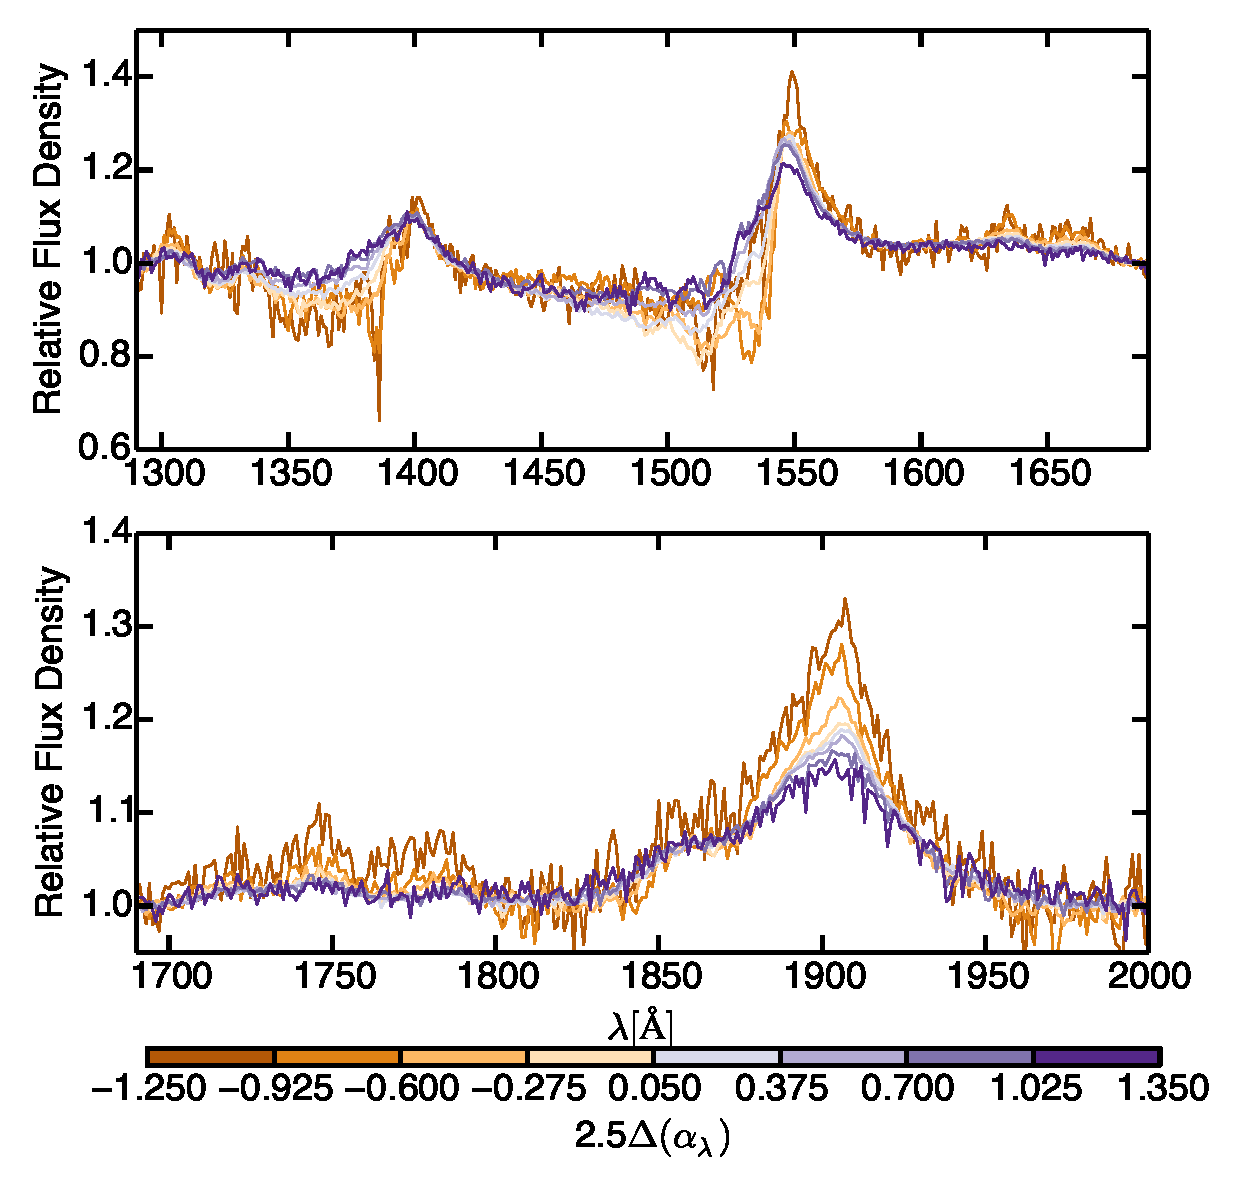
\includegraphics[width=4.5in]{images/Dust/f15}
\caption[Expanded emission-line regions for BAL quasars]{\label{fig:ind_bal_spec} Expanded emission-line regions from the lowest $\ebv$ bin from Figure~\ref{fig:bal_spec} ($0.012<\ebv<0.044$). The colors represent the 2.5$\dal$ value for each spectrum.  The spectra are normalized such that their continua agree at the edges of the panels. Intrinsically redder BALs have stronger \ion{C}{4} and \ion{C}{3}] emission lines.  The correlation see between changes in both the emission and absorption lines indicate they are both responding to changes in the underlying SED.}
\end{center}
\end{figure}

We also looked at the same spectral lines while holding 2.5$\dal$ fixed and comparing spectra with different value of $\ebv$.  The clearest trend is seen in \ion{C}{4}, where the strength of the line decreases as the reddening increases.  Unlike \citet{Richards:2003} we do not see any increase in the strength of [\ion{O}{2}] with reddening, but we do see a slight increase in the [\ion{O}{3}] lines. The strong increase in [\ion{O}{2}] seen in \citet{Richards:2003} could have been caused by intrinsically red quasars being mistaken as dust reddened in their sample.

%When studying the same spectral lines when holding the intrinsic color fixed and comparing different value for $\ebv$ find very different results than \citet{Richards:2003}.
%In Figure~\ref{fig:ind_spec2} we show the same spectral lines, this time holding the intrinsic color fixed ($0.05<\dal<0.38$) and showing different values for $\ebv$.  Like in Figure~\ref{fig:ind_spec} we choose a subset from each bin such that the $L_{2500\,\AA}$ distribution is the same for each spectra\footnote{We used the observed luminosity not corrected for reddening}. 
%The clearest trend is seen in \ion{C}{4}, where the strength and blueshift of the line both decrease as the reddening increase.  Unlike \citet{Richards:2003} we do not see any increase in the strength of [\ion{O}{2}] with reddening, but we do see an increase in the [\ion{O}{3}] lines.  The strong increase in [\ion{O}{2}] seen in \citet{Richards:2003} could have been caused by intrinsically red quasars being mistaken as dust reddened in their sample.

In the BAL spectra we confirm differences in the emission and (mean) absorption as a function of (intrinsic) color (see Figure~\ref{fig:ind_bal_spec}), with the redder objects having more strongly peaked \ion{C}{4}, stronger \ion{C}{3} (and \ion{Si}{3}) and some excess at $\sim$1750\,\AA, as was seen in Figure 9 of \citet{Reichard:2003b}. The absorption and emission are correlated as might be expected if both are responding to differences in the SED.  If the absorption was not responding to differences in the SED, the differences in the absorption troughs would be averaged away and little variation would be seen in the composites. Therefore, the correlation that we see indicates there may be some underlying trend relating both the absorption and emission \citep[e.g.,][]{Turnshek:1988}.  The narrow, low-velocity absorption seen in the redder BAL quasars (just blueward of the \ion{C}{4} and \ion{Si}{4} lines) could be an indication of weaker wind or a higher column density.  These quasars also show evidence of strong, not blueshifted \ion{C}{4} and strong \ion{C}{3}] two properties that \citet{Richards:2011} argue are also indicators of a weaker winds.

We note that radio-loud (RL) ``BALs'' \citet[e.g.,][]{Becker:2000} do not always meet the formal definition of BALs, having relatively weak absorption troughs at low velocity. As the RL quasars tend to be (on average) redder than radio-quiet (RQ) quasars, our finding of mini-BAL-like residuals in the reddest composites may not be that surprising. 

%[RL quasars also intrinsically redder.  So this could be consistent with the BALs in the redder objects being mini-BALs as opposed to troughs that meet the classical BAL definition.]
%[cmk: not sure I follow the connection between RL and mini-BALs]

\section{Conclusions} \label{sec:conclusions}

Using mid-IR thorough UV photometry alone we calculated intrinsic powerlaw slopes (2.5$\dal$) and SMC reddening law coefficients ($\ebv$) for $\sim$35,000 uniformly selected quasars from the SDSS DR7 quasar catalog.  By using a hierarchical Bayesian model we were able to break the degeneracy between these parameters and keep both of them in a physical range (Figure~\ref{fig:indv_fits_SMC}). From these fits we found that BAL quasars are biased (blueward) within the parent population as compared to the non-BAL quasars.
%that non-BAL and BAL quasars do not have the same parent population.  
Both the BAL and non-BAL quasars are bluer than the modal spectral index ($\alpha_\lambda = -1.83$ and -1.79 respectively) while the BAL quasars have higher amounts of reddening (13\% with $\ebv>0.1$) than the non-BAL quasars (2.5\% with $\ebv>0.1$).
%The BAL quasars are slightly bluer ($\alpha_\lambda = -1.83$) and have higher amounts of reddening (13\% with $\ebv>0.1$) than the non-BAL quasars ($\alpha_\lambda = -1.79$, 2.5\% with $\ebv>0.1$).  
We also find the BAL fraction is very dependent on the intrinsic color and amount of dust reddening of the quasars.  After marginalizing over $\ebv$ we find the {\em observed} BAL fraction increases from $\sim$0.05 to $\sim$0.2 as quasars become bluer (Figure~\ref{fig:bal_frac}). 
%The conjunction of high BAL fraction with extremely blue intrinsic continua and large $\ebv$ values implies that in these objects the BAL wind covers a large fraction of the sky.
%[Still something fishy there.   How many BALs and non-BALs are you studying? Also need to put back the objects with absorption lines when doing this.]

We constructed composite spectra by splitting the resulting measurements of 2.5$\dal$ and $\ebv$ into a 10x10 grid. With the exception of the non-BAL quasars with the most reddening and the bluest quasars with the least reddening, the fit values for each bin do a good job of reproducing the slopes and curvatures of the spectra, showing that our fit values are consistent with being physically meaningful (Figures~\ref{fig:spec} and~\ref{fig:bal_spec}). Exploring the spectra further, we found within the BAL sample that the \ion{C}{4} absorption trough becomes deeper as $\ebv$ increases and becomes wider as quasars become bluer.
%Exploring the spectra further, we found that the highly reddened BAL quasars are dominated by LoBALs while the less reddened sample is dominated by HiBALs.  This trend is in agreement with many previous studies \citep[e.g., ][]{Weymann:1991,Reichard:2003a,Reichard:2003b}, and is consistent with the orientation-dependent picture presented in \citet{Weymann:1991}.

Comparing the spectra in the lowest reddening bin revealed trends in the spectral lines based on a quasar's intrinsic color.  We found that intrinsically red quasars have stronger \ion{C}{4}, \ion{He}{2}, \ion{C}{3}], and [\ion{O}{2}], while the \ion{Mg}{2}, H$\gamma$, H$\beta$, H$\alpha$, and the SBB are all weaker (Figure~\ref{fig:ind_spec}).  
These stronger ionization lines in the intrinsically red quasars indicate that they have more ionizing photons (harder SED) in the energy range $\sim$13.6--64.5\,eV (15.5$\lesssim\log{(\nu [Hz])}\lesssim$16.2) than the bluer quasars. Additionally, the width of H$\beta$ and \ion{Mg}{2} are proportional to the mass of the central black hole, indicating that the bluer quasars likely have larger $\mbh$.  Or if H$\beta$ is used as an indicator of inclination, the bluer quasars might be instead viewed closer to edge-on.
%or have host galaxy contamination that is a function of color.  
We will take a closer look at these trends in Chapter~\ref{BH}.
%When holding the intrinsic color fixed and looking at spectra with different amounts of reddening, we only see trends in \ion{C}{4} (weaker for more reddened quasars) and [\ion{O}{3}] (stronger for more reddened quasars). 
In the BAL sample similar trends were found in \ion{C}{3}] and \ion{C}{4} (stronger for redder quasars), and in addition we see that the absorption troughs are responding to the changes in the underlying SED (Figure~\ref{fig:ind_bal_spec}).
%that the depth of the \ion{C}{4} and \ion{Si}{4} BAL troughs are more consistent for redder quasars (Figure~\ref{fig:ind_bal_spec}).